
%DIF LATEXDIFF DIFFERENCE FILE
%DIF DEL main_former.tex   Mon Feb  7 14:29:35 2022
%DIF ADD main.tex          Mon Feb 14 17:17:53 2022
\newif\ifIEEEversion % turn on IEEE style 
\IEEEversiontrue
\newif\ifanon % needed for acks, suppression of authors, etc
\anontrue


\ifIEEEversion
%% what follows is for the IEEEtran format required for IEEE Euro S&P

\documentclass[compsoc,conference,a4paper,10pt,times]{IEEEtran}

%% our own choice of packages 
\usepackage{graphicx, amsmath, amsthm, amssymb, setspace, array, url, xspace, todonotes, pifont} %hyperref is supplied by IEEEtran below
%\usepackage{a4wide}
\usepackage[utf8]{inputenc}
\usepackage[T1]{fontenc}
\newcommand{\cmark}{\ding{51}}%
\newcommand{\xmark}{\ding{55}}%

%% packages and whatnot inherited from IEEEtran example file

\IEEEoverridecommandlockouts
% The preceding line is only needed to identify funding in the first footnote. If that is unneeded, please comment it out.
\usepackage{cite}
\usepackage{amsmath,amssymb,amsfonts}
\usepackage{algorithmic}
\usepackage{graphicx}
\usepackage{textcomp}
\usepackage{bmpsize}
\usepackage{xcolor}
\usepackage{lipsum}
\usepackage[colorlinks=true,urlcolor=black]{hyperref}
%% commented out this nonsense
%\def\BibTeX{{\rm B\kern-.05em{\sc i\kern-.025em b}\kern-.08em
%   T\kern-.1667em\lower.7ex\hbox{E}\kern-.125emX}}
%% need these for IEEEtran - not defined in cls file
\newtheorem{lemma}{Lemma}
\newtheorem{theorem}{Theorem}
\newtheorem{definition}{Definition}
%DIF PREAMBLE EXTENSION ADDED BY LATEXDIFF
%DIF UNDERLINE PREAMBLE %DIF PREAMBLE
\RequirePackage[normalem]{ulem} %DIF PREAMBLE
\RequirePackage{color}\definecolor{RED}{rgb}{1,0,0}\definecolor{BLUE}{rgb}{0,0,1} %DIF PREAMBLE
\providecommand{\DIFaddtex}[1]{{\protect\color{blue}\uwave{#1}}} %DIF PREAMBLE
\providecommand{\DIFdeltex}[1]{{\protect\color{red}\sout{#1}}}                      %DIF PREAMBLE
%DIF SAFE PREAMBLE %DIF PREAMBLE
\providecommand{\DIFaddbegin}{} %DIF PREAMBLE
\providecommand{\DIFaddend}{} %DIF PREAMBLE
\providecommand{\DIFdelbegin}{} %DIF PREAMBLE
\providecommand{\DIFdelend}{} %DIF PREAMBLE
\providecommand{\DIFmodbegin}{} %DIF PREAMBLE
\providecommand{\DIFmodend}{} %DIF PREAMBLE
%DIF FLOATSAFE PREAMBLE %DIF PREAMBLE
\providecommand{\DIFaddFL}[1]{\DIFadd{#1}} %DIF PREAMBLE
\providecommand{\DIFdelFL}[1]{\DIFdel{#1}} %DIF PREAMBLE
\providecommand{\DIFaddbeginFL}{} %DIF PREAMBLE
\providecommand{\DIFaddendFL}{} %DIF PREAMBLE
\providecommand{\DIFdelbeginFL}{} %DIF PREAMBLE
\providecommand{\DIFdelendFL}{} %DIF PREAMBLE
%DIF HYPERREF PREAMBLE %DIF PREAMBLE
\providecommand{\DIFadd}[1]{\texorpdfstring{\DIFaddtex{#1}}{#1}} %DIF PREAMBLE
\providecommand{\DIFdel}[1]{\texorpdfstring{\DIFdeltex{#1}}{}} %DIF PREAMBLE
\newcommand{\DIFscaledelfig}{0.5}
%DIF HIGHLIGHTGRAPHICS PREAMBLE %DIF PREAMBLE
\RequirePackage{settobox} %DIF PREAMBLE
\RequirePackage{letltxmacro} %DIF PREAMBLE
\newsavebox{\DIFdelgraphicsbox} %DIF PREAMBLE
\newlength{\DIFdelgraphicswidth} %DIF PREAMBLE
\newlength{\DIFdelgraphicsheight} %DIF PREAMBLE
% store original definition of \includegraphics %DIF PREAMBLE
\LetLtxMacro{\DIFOincludegraphics}{\includegraphics} %DIF PREAMBLE
\newcommand{\DIFaddincludegraphics}[2][]{{\color{blue}\fbox{\DIFOincludegraphics[#1]{#2}}}} %DIF PREAMBLE
\newcommand{\DIFdelincludegraphics}[2][]{% %DIF PREAMBLE
\sbox{\DIFdelgraphicsbox}{\DIFOincludegraphics[#1]{#2}}% %DIF PREAMBLE
\settoboxwidth{\DIFdelgraphicswidth}{\DIFdelgraphicsbox} %DIF PREAMBLE
\settoboxtotalheight{\DIFdelgraphicsheight}{\DIFdelgraphicsbox} %DIF PREAMBLE
\scalebox{\DIFscaledelfig}{% %DIF PREAMBLE
\parbox[b]{\DIFdelgraphicswidth}{\usebox{\DIFdelgraphicsbox}\\[-\baselineskip] \rule{\DIFdelgraphicswidth}{0em}}\llap{\resizebox{\DIFdelgraphicswidth}{\DIFdelgraphicsheight}{% %DIF PREAMBLE
\setlength{\unitlength}{\DIFdelgraphicswidth}% %DIF PREAMBLE
\begin{picture}(1,1)% %DIF PREAMBLE
\thicklines\linethickness{2pt} %DIF PREAMBLE
{\color[rgb]{1,0,0}\put(0,0){\framebox(1,1){}}}% %DIF PREAMBLE
{\color[rgb]{1,0,0}\put(0,0){\line( 1,1){1}}}% %DIF PREAMBLE
{\color[rgb]{1,0,0}\put(0,1){\line(1,-1){1}}}% %DIF PREAMBLE
\end{picture}% %DIF PREAMBLE
}\hspace*{3pt}}} %DIF PREAMBLE
} %DIF PREAMBLE
\LetLtxMacro{\DIFOaddbegin}{\DIFaddbegin} %DIF PREAMBLE
\LetLtxMacro{\DIFOaddend}{\DIFaddend} %DIF PREAMBLE
\LetLtxMacro{\DIFOdelbegin}{\DIFdelbegin} %DIF PREAMBLE
\LetLtxMacro{\DIFOdelend}{\DIFdelend} %DIF PREAMBLE
\DeclareRobustCommand{\DIFaddbegin}{\DIFOaddbegin \let\includegraphics\DIFaddincludegraphics} %DIF PREAMBLE
\DeclareRobustCommand{\DIFaddend}{\DIFOaddend \let\includegraphics\DIFOincludegraphics} %DIF PREAMBLE
\DeclareRobustCommand{\DIFdelbegin}{\DIFOdelbegin \let\includegraphics\DIFdelincludegraphics} %DIF PREAMBLE
\DeclareRobustCommand{\DIFdelend}{\DIFOaddend \let\includegraphics\DIFOincludegraphics} %DIF PREAMBLE
\LetLtxMacro{\DIFOaddbeginFL}{\DIFaddbeginFL} %DIF PREAMBLE
\LetLtxMacro{\DIFOaddendFL}{\DIFaddendFL} %DIF PREAMBLE
\LetLtxMacro{\DIFOdelbeginFL}{\DIFdelbeginFL} %DIF PREAMBLE
\LetLtxMacro{\DIFOdelendFL}{\DIFdelendFL} %DIF PREAMBLE
\DeclareRobustCommand{\DIFaddbeginFL}{\DIFOaddbeginFL \let\includegraphics\DIFaddincludegraphics} %DIF PREAMBLE
\DeclareRobustCommand{\DIFaddendFL}{\DIFOaddendFL \let\includegraphics\DIFOincludegraphics} %DIF PREAMBLE
\DeclareRobustCommand{\DIFdelbeginFL}{\DIFOdelbeginFL \let\includegraphics\DIFdelincludegraphics} %DIF PREAMBLE
\DeclareRobustCommand{\DIFdelendFL}{\DIFOaddendFL \let\includegraphics\DIFOincludegraphics} %DIF PREAMBLE
%DIF LISTINGS PREAMBLE %DIF PREAMBLE
\RequirePackage{listings} %DIF PREAMBLE
\RequirePackage{color} %DIF PREAMBLE
\lstdefinelanguage{DIFcode}{ %DIF PREAMBLE
%DIF DIFCODE_UNDERLINE %DIF PREAMBLE
  moredelim=[il][\color{red}\sout]{\%DIF\ <\ }, %DIF PREAMBLE
  moredelim=[il][\color{blue}\uwave]{\%DIF\ >\ } %DIF PREAMBLE
} %DIF PREAMBLE
\lstdefinestyle{DIFverbatimstyle}{ %DIF PREAMBLE
	language=DIFcode, %DIF PREAMBLE
	basicstyle=\ttfamily, %DIF PREAMBLE
	columns=fullflexible, %DIF PREAMBLE
	keepspaces=true %DIF PREAMBLE
} %DIF PREAMBLE
\lstnewenvironment{DIFverbatim}{\lstset{style=DIFverbatimstyle}}{} %DIF PREAMBLE
\lstnewenvironment{DIFverbatim*}{\lstset{style=DIFverbatimstyle,showspaces=true}}{} %DIF PREAMBLE
%DIF END PREAMBLE EXTENSION ADDED BY LATEXDIFF

\begin{document}

\title{HyperLogLog: Exponentially Bad in Adversarial Settings}

\ifanon %% suppress authors in anonymous version
\author{}
\else
\author{\IEEEauthorblockN{Kenneth G. Paterson}
\IEEEauthorblockA{\textit{ETH Zurich} \\
kenny.paterson@inf.ethz.ch}
\and
\IEEEauthorblockN{Mathilde Raynal}
\IEEEauthorblockA{\textit{EPFL} \\
mathilde.raynal@epfl.ch}
}
\fi %end anon processing of authors

\else  %% what follows is a vanilla format for posting on eprint

\documentclass[a4paper,10pt]{article}

%% our own choice of packages 
\usepackage{graphicx, amsmath, amsthm, amssymb, setspace, array, url, xspace, todonotes, pifont, hyperref} 
\usepackage{a4wide}
%\usepackage{authblk}
\usepackage[utf8]{inputenc}
\usepackage[T1]{fontenc}
\newcommand{\cmark}{\ding{51}}%
\newcommand{\xmark}{\ding{55}}%
\newtheorem{lemma}{Lemma}
\newtheorem{theorem}{Theorem}
\newtheorem{definition}{Definition}

\begin{document}

\title{HyperLogLog: Exponentially Bad in Adversarial Settings}
\ifanon %% suppress authors in anonymous version
\author{}
\else
\author{Kenneth G. Paterson\\ETH Zurich\\\texttt{kenny.paterson@inf.ethz.ch} \and Mathilde Raynal\\EPFL\\\texttt{mathilde.raynal@epfl.ch}}
\fi % end anon processing of authors 
\fi % end of vanilla format 

\maketitle


\begin{abstract}
Computing the count of distinct elements in large data sets is a common task but naive approaches are memory-expensive. The HyperLogLog (HLL) algorithm (Flajolet \emph{et al.}, 2007) estimates a data set's cardinality while using significantly less memory than a naive approach, at the cost of some accuracy. This trade-off makes the HLL algorithm very attractive for a wide range of applications such as database management and network monitoring, where an exact count may not be needed. The HLL algorithm and variants of it are implemented in systems such as Redis and Google Big Query. Recently, the HLL algorithm has started to be proposed for use in scenarios where the inputs may be adversarially generated, for example counting social network users or detection of network scanning attacks. This prompts an examination of the performance of the HLL algorithm in the face of adversarial inputs. We show that in such a setting, the HLL algorithm's estimate of cardinality can be exponentially bad: when an adversary has access to the internals of the HLL algorithm and has some flexibility in choosing what inputs will be recorded, it can manipulate the cardinality estimate to be exponentially smaller than the true cardinality. We study both the original HLL algorithm and a more modern version of it (Ertl, 2017) that is used in Redis. We present experimental results confirming our theoretical analysis. Finally, we consider attack prevention: we show how to modify HLL in a simple way that provably prevents cardinality estimate manipulation attacks.
\end{abstract}

%\begin{IEEEkeywords}
%yadda yadda
%\end{IEEEkeywords}

\section{Introduction}
Data scientists today make use of systems like Google Big Query, Apache Spark, Presto and Redis to handle large data sets. Such systems include analytics engines capable of performing powerful operations on the data. Particularly useful to data scientists are summary statistics, with a key statistic being the number of distinct data items in a data set, i.e.\ the data set's cardinality. In many use cases, obtaining an approximate cardinality is sufficient. Over the last decade, the HyperLogLog (HLL) cardinality estimator~\cite{hll} has emerged as the algorithm of choice for this task, due to its excellent speed, low memory requirements and high proven accuracy.\footnote{Section~\ref{sec:overview} contains a complete specification of HLL.} It is also suitable for use in applications where it is not possible (or desirable) to store an entire data set, but instead where the data set is presented in a streaming fashion. HLL is used by all of the above-mentioned systems.

However, HLL is increasingly used in settings where adversaries may have incentives to manipulate the cardinality estimates made by the algorithm, i.e.\ HLL is being used in \emph{adversarial settings}. For example:
\begin{itemize}
    \item Facebook uses HLL to find out how many distinct people visited their website in the past week~\cite{fbhll}.
    \item Google uses a variant of HLL described in~\cite{hllpractice} in its PowerDrill system (first described in~\cite{HallBBGN12}) and possibly in a variety of other internal systems reported in~\cite{hllpractice}. For example, cardinality estimation is used to determine the number of distinct search queries on \url{google.com} over a time period~\cite{hllpractice}. %HLL is also used for cardinality estimation via an API in Google Big Query. 
    \item HLL has been implemented in network soft-switches to approximate the number of distinct packets in traffic flows and overcome the switch memory limits~\cite{flexswitch}. The number of unique flows traversing a switch is then used to  inform a congestion control mechanism.
    \item HLL has been proposed as a solution to detecting Denial-of-Service attacks~\cite{portscanhll} (this paper actually uses a variation on HLL called \emph{sliding HLL}~\cite{slidinghll} which estimates the cardinality over a moving time window). Specifically, HLL is used to count how many different destination ports are seen over all packets received, in an attempt to identify when a port scan attack is underway.
\end{itemize}

None of the above-cited examples discuss any kind of threat model where an adversary may try to manipulate the HLL cardinality estimate to its advantage. This is despite them all operating in potentially adversarial settings. We infer that the developers of these systems may not be fully aware of the risks they are taking in relying on HLL.

Recently, Reviriego and Ting~\cite{hllvuln} initiated work on the performance of HLL in adversarial settings. They showed that in very specific attack settings, the cardinality estimate made by HLL can be modified through input selection. In this paper, we present a complete analysis of HLL in adversarial settings, considering more realistic attack scenarios and giving more powerful attacks than~\cite{hllvuln}. In particular, we show that with only modest knowledge of the HLL internals and a moderate amount of computation, an adversary with sufficient flexibility in the choice of inputs can make the HLL cardinality estimate exponentially smaller than the true cardinality (e.g.\ constant instead of ${\mathcal{O}}(2^t)$ where $t$ is the number of bits of flexibility in the adversary's input). We demonstrate this theoretically and experimentally for the ``classic'' version of HLL from~\cite{hll}. We also study a specific ``modern'' version of HLL which adopts recommendations from~\cite{hllnew} and show how variants of our attacks apply there too. This modern version of HLL is interesting because it is the one used in Redis.

We stress that none of our attacks are particularly deep in cryptanalytic terms. \DIFaddbegin \DIFadd{Fundamentally, they arise from implementations of HLL using a fixed hash function $h$ internally. }\DIFaddend Yet HLL is being increasingly widely deployed, and never with protections against our attacks (insofar as we are aware). So despite their technical simplicity, we argue that our attacks are important in establishing the limitations of HLL in the broadest set of use cases. We present our attacks in an abstract way rather than tying them to any specific setting in order to illustrate their generality. We do give a more detailed exploration of their impact on the data-centre network monitoring system proposed in~\cite{flexswitch}, see Section~\ref{sec:exp}. 

To complement our attack results, we provide a formal security analysis of HLL. We show that in the ``shadow device'' attack scenario of~\cite{hllvuln}, no security is possible even if HLL is secretly keyed. On the other hand, we also show that in the most powerful attack setting introduced here, where the attacker has full access to the internals of the HLL algorithm (except for a secret key!), it is possible to provably secure HLL against cardinality manipulation by the simple expedient of replacing its internal hash function $h$ by a keyed, variable-input-length pseudo-random function (VIL-PRF) $F$. We discuss and benchmark a suitable choice for the required VIL-PRF. To support our formal analysis, we introduce a novel simulation-based security model for HLL. We believe our simulation-based approach will be of independent interest and will be useful beyond the analysis of cardinality manipulation attacks, for example when studying privacy properties of HLL and other probabilistic data structures. 

\DIFaddbegin \subsection{\DIFadd{Potential Harms and Mitigations}}\label{sec-harms}

\DIFadd{Our attacks are presented in a general way and evaluated either abstractly or in the context of a specific system described in the scientific literature~\mbox{%DIFAUXCMD
\cite{flexswitch}}\hspace{0pt}%DIFAUXCMD
. We also propose an easily deployable countermeasure. Given this, we think the potential for harm to systems and individuals relying on HLL today is small. On the other hand, we hope our results will spur practitioners to consider the possibility of adversarial inputs in their specific applications and design accordingly. For the specific case of Redis, a real system that we analyse in detail, we have contacted the Redis core team and shared our results, following their advertised security policy.}\footnote{\url{https://github.com/redis/redis/security/policy}\DIFadd{.}}

\DIFaddend \subsection{Paper Organisation}
The rest of the paper is organised as follows. Section~\ref{sec:related} immediately below discusses related work. Section~\ref{sec:overview} gives an overview of HLL. Section~\ref{sec:attacks} \DIFaddbegin \DIFadd{informally }\DIFaddend presents our different adversarial models. In Section~\ref{sec:manip}, we describe attacks on HLL and evaluate their impacts under the different adversarial models. Section~\ref{sec:redis} considers the security of the more modern version of HLL due to Ertl~\cite{hllnew} that is used in Redis. Our experimental results are discussed and related back to a specific application setting in Section~\ref{sec:exp}. Section~\ref{sec:formal} provides our formal security \DIFdelbegin \DIFdel{analysis of HLL }\DIFdelend \DIFaddbegin \DIFadd{model and security proof for HLL using a VIL-PRF}\DIFaddend . Section~\ref{sec:conclusions} provides our conclusions and ideas for future work.

\section{Related Work}\label{sec:related}

Desfontaines \emph{et al.}~\cite{cardestprivacy} studied the privacy properties of HLL in two different attack scenarios, referred to as \emph{insider} and \emph{external}. The attack target of~\cite{cardestprivacy} is different from ours, being focused on privacy breaches. %It is argued in~\cite{cardestprivacy} that HLL can be used by organisations to store and process location data, which is inherently sensitive, so losing privacy would leak users' locations and potentially cause great harm. In contrast, we are concerned with an attacker attempting to manipulate the cardinality estimation process itself (an issue not considered in~\cite{cardestprivacy}).
We discuss the two attack scenarios from~\cite{cardestprivacy} in more detail in Section~\ref{sec:attacks}. 

In~\cite{hllvuln}, Reviriego and Ting exploit a vulnerability of HLL to manipulate the cardinality estimate, leading to a five-fold reduction in the estimate compared to the true cardinality. We consider the attack model used in~\cite{hllvuln} to be quite artificial, since it gives the adversary the ability to test whether inserting an item \emph{would} increase the cardinality estimate, without actually having to insert the item. Such a setup might be possible under certain circumstances, for example where the adversary has access to an identical ``shadow'' device; see further discussion in Section~\ref{sec:attacks}. For completeness, we include analyses of this attack scenario, showing that we can drastically improve on the attacks in~\cite{hllvuln} (e.g.\ we can reduce the HLL cardinality estimate by a factor of almost 1,000 instead of the factor of 5 achieved in~\cite{hllvuln}). However, we stress that we consider this scenario to be the least realistic (and therefore the least interesting).

Both~\cite{cardestprivacy,hllvuln} propose mitigations using a salted HLL sketch, either as a replacement for (but at the cost of losing mergeability) or in addition to (inducing a memory overhead) an unsalted HLL. We show in Section~\ref{sec:formal} that when a salt is used appropriately (i.e.\ as the secret key for a pseudo-random function that is used in place of hash function $h$), security against adversarial inputs can be achieved even in our strongest adversarial setting. \DIFaddbegin \DIFadd{However, this comes at the cost of losing mergeability. 
}\DIFaddend %In addition, our simulation-based security definition, in which the simulator in the ideal world has no access to the inserted values, automatically guarantees confidentiality of the values inserted into the HLL sketch, even in the strongest attack model considered in~\cite{cardestprivacy}. So, while our main objective is to protect against adversarial inputs, we also get privacy for free when using a keyed PRF in place of the HLL hash function. 

Our work relates to the broader study of the performance of probabilistic data structures in adversarial environments.
Clayton \emph{et al.}~\cite{CCS:ClaPatShrPS19} recently provided a provable-security treatment of this topic. They used a game-based formalism to analyze Bloom filters, counting (Bloom) filters and count-min sketch data structures. They did not study HLL. Our use of a simulation-based security definition in place of the game-based ones used in~\cite{CCS:ClaPatShrPS19} is another point of distinction; see further discussion in Section~\ref{sec:formal}. Prior work also focused on Bloom filters~\cite{NaorY15,GerbetKL15} or flooding of hash tables~\cite{LiptonN93,CrosbyW03}. %References~\cite{GerbetKL15,CCS:ClaPatShrPS19} provide summaries of prior work in this area. 
Recent papers~\cite{Ben-EliezerJWY20,DBLP:journals/corr/abs-2011-07471,HassidimKMMS20,KaplanMNS21} have studied broad classes streaming algorithms under adversarial input from a theoretical viewpoint. Our applied \DIFdelbegin \DIFdel{viewpoint }\DIFdelend \DIFaddbegin \DIFadd{perspective }\DIFaddend complements this work, focussing on the real-world usage of a specific cardinality estimator. 
%The authors of~\cite{Ben-EliezerJWY20} give a compiler that shows how to generically transform a non-robust streaming algorithm into a robust one in various scenarios. For the particular case of cardinality estimation, this results in solutions that are much less efficient than ours using a PRF; the security model used in this line of work is also weaker than our strongest model.

\section{Overview of HLL}\label{sec:overview}

\begin{figure*}[tb!]
\centering
\caption{ \DIFaddbegin \DIFadd{The HyperLogLog Algorithm from~\cite{hll}}\DIFaddend}
     \makebox[\linewidth]{
\fbox{
\begin{minipage}{40em}
\begin{flushleft}
\textit{Let $h : \hat{\mathcal{D}} \rightarrow \{0, 1\}^{32}$ hash data from some domain $\hat{\mathcal{D}}$ to binary $32$-bit strings.\\
For $s$ of bit-length $\ell$, let $\rho(s)$ denote the position of the leftmost $1$-bit of $s$: e.g., $\rho(1...) = 1, \rho(0001...) = 4, \rho(0^\ell) = \ell + 1.$\\}
\textbf{define} $m = 2^n$ with $n \in [4..16].$\\
\textbf{define} $\alpha_{16} = 0.673$; $\alpha_{32} = 0.697$; $\alpha_{64} = 0.709$; $\alpha_{m} = 0.7213/(1+ 1.079/m)$ for $m \ge 128$;\\
\vspace{0.5em}
\textbf{Algorithm} HyperLogLog (\textbf{input} ${\mathcal{X}}$ : multiset of items from domain $\hat{\mathcal{D}}$).\\
\textbf{initialize} a collection of $m$ registers, $M[1], ..., M[m]$, to $0$;\\
\vspace{0.5em}
\textbf{for} $x \in {\mathcal{X}}$ \textbf{do}\\
    \hspace{2em} \textbf{set} $y := h(x);$\\
    \hspace{2em} \textbf{set} $j = 1 + <y_1y_2...y_{n}>_2$; \hfill \textit{\{bucket index determined by the first $n$ bits of $y$\}}\\
    \hspace{2em} \textbf{set} $w := y_{n+1}y_{n+2} \ldots y_{n+\ell}$;\hfill \textit{\{bit string determined by the last $\ell$ bits of $y$\}}\\
   \hspace{2em} \textbf{set} $M[j] :=$ max$(M[j], \rho(w))$;\\
\vspace{0.2em}
\textbf{compute} $E := \alpha_mm^2\cdot(\sum_{j=1}^m2^{-M[j]})^{-1}$; \hfill \textit{\{the raw HyperLogLog estimate\}}\\
\vspace{0.2em}
\textbf{if} $E \le \frac{5}{2}m$ \textbf{then}\\
    \hspace{2em}  \textbf{let} $V$ be the number of registers equal to $0$;\\
    \hspace{2em}  \textbf{if} $V \neq 0$ \textbf{then set} $E^*:=  m\cdot \ln(m/V)$ \textbf{else set} $E^*:= E$; \hfill \textit{\{small range correction\}}\\
\textbf{if} $E \le \frac{1}{30}2^{32}$ \textbf{then}\\
    \hspace{2em} \textbf{set} $E^*:= E$; \hfill \textit{\{intermediate range --- no correction\}}\\
\textbf{if} $E > \frac{1}{30}2^{32}$ \textbf{then}\\
    \hspace{2em}  \textbf{set} $E^*:= -2^{32}\ln(1 - E/2^{32})$; \hfill \textit{\{large range correction\}}\\
\textbf{return} \textit{cardinality estimate $E^*$ with typical relative error} $\pm1.04/\sqrt{m}$.
\end{flushleft}
\end{minipage}
}}
 \DIFdelbegin \DIFdel{The HyperLogLog Algorithm from~\cite{hll}}\DIFdelend
\label{fig:hll}
\end{figure*}


HLL~\cite{hll} is based on the key observation that, for a stream of items represented as bit-strings of some fixed length, if all items have at most $k$ leading zero-bits (and one or more items actually have this many leading zero-bits), then the cardinality of the stream (i.e.\ the number of distinct values it contains) is likely to be on the order of $2^{k+1}$. To ensure a uniform distribution on the items' representations as bit-strings, the items are processed by a hash function $h$ before the leading bits are inspected.

So to roughly estimate the cardinality of a stream, we need only to store a representation of $k$, the length of the largest observed string of leading zero-bits for hashes of items in the stream. This provides a very compact mechanism for estimating a stream's cardinality -- if the true cardinality is $N$, then just \DIFdelbegin \DIFdel{$\mathcal{O}(\log\log(N))$ }\DIFdelend \DIFaddbegin \DIFadd{$\mathcal{O}(\log_2\log_2(N))$ }\DIFaddend bits of storage are needed to compute the cardinality estimate.

This simple approach suffers from large variance. In order to reduce the variance, HLL uses many estimators in parallel instead of one and averages the results. Each estimate is stored in its own register that we call a bucket. We refer to the collection of buckets and their contents as the HLL \emph{sketch}. To map a value $x$ to one of $m=2^n$ buckets, \cite{loglog} suggests using the first $n$ bits of $h(x)$ as a bucket index, and then computing the longest sequence of leading zero bits on the remaining $\ell$ bits of $h(x)$. The output length of $h(\cdot)$ is thus $n+\ell$. This sum is fixed to 32 in the original HLL paper~\cite{hll}. Estimates from all buckets are averaged using the harmonic mean and scaled by a constant $\alpha_m$, where $\alpha_m$ is empirically computed to correct a systematic multiplicative bias. See Figure~\ref{fig:hll}.

In the original HLL proposal~\cite{hll}, relatively small and large cardinalities are handled separately to correct for systematic errors. When the raw cardinality estimate is below $\frac{5}{2}m$, the Hit Counting algorithm of Whang \emph{et al.}~\cite{hitcounting} is used to produce the final cardinality estimate. This estimator uses the number of empty buckets (whose register value is 0) instead of the number of leading zeros in the stream. A similar correction is applied for large cardinalities in order to take into account the likelihood of hash collisions. In addition, the cardinality estimate is usually rounded to a whole number before being output. The original HLL algorithm from~\cite{hll} is shown in Figure~\ref{fig:hll}. This algorithm is able to estimate cardinalities greater than $10^9$ with a typical standard error of 4\%, using only 1.5 kB of memory. Crucially, the proof of this~\cite[Theorem 1]{hll} makes the assumption that the inputs are drawn independently and uniformly at random from the input domain -- loosely put, it is an average case analysis.\footnote{Technically, the results of~\cite{hll} are proven for a distribution obtained by making arbitrary replications and permutations after sampling independently and uniformly, to simulate input taken from an \emph{ideal multiset}. But they also hold without replication and permutation because HLL's internal state is invariant under repeated inputs.}

Some works building on~\cite{hll} replace the Hit Counting algorithm by other schemes and use a hash function with a larger output domain to reduce the chances of collision and thus get rid of the need for large cardinality range correction. For example, Google engineers proposed using a 64-bit hash function and Linear Counting along with bias correction in the small cardinality range~\cite{hllpractice},\footnote{See also the Google blogpost describing the implementation in Google Big Query at~\url{https://cloud.google.com/blog/products/gcp/counting-uniques-faster-in-bigquery-with-hyperloglog}.} while Redis has adopted a new estimator based on a more precise statistical analysis of the counting problem provided by~\cite{hllnew}. 

In this paper we mostly focus on the HLL formulation in the original paper~\cite{hll} as represented in Fig.~\ref{fig:hll} and as widely used in practice. We also study~\cite{hllnew} because of its recent deployment in Redis.  We leave for future work the analysis of further HLL variants. %\todo{revise this if we add Google BQ.}

An interesting property of HLL is that it supports merging in a lossless way. To combine two buckets at index $i$ in two different HLL instances, one can take the maximum of the two bucket entries and assign that to the matching bucket $i$ in the merged HLL sketch. Such a simple set union operation allows easy parallelisation of operations among multiple machines independently, provided they use the same hash function and the same number of buckets. Clearly this procedure cannot be carried out if the different HLL sketches are differently seeded or keyed.

\section{HLL in Adversarial Settings}\label{sec:attacks}

This section presents the different adversarial settings that we consider. In all settings, our adversary's aim is to manipulate the HLL cardinality estimate. We focus on reducing the estimate as much as possible, since this would cause more damage when  considering the previously mentioned applications of HLL. It is easy to modify our attack strategies for an adversary who instead wishes to artificially inflate the HLL cardinality estimate given a limited input capability. 
%We also analyze the impact on the HLL cardinality estimate and the computational effort required.

\subsection{Attacker's Objective, Abstractly}
Throughout, we assume the adversary has the ability to vary the contents of free fields in the strings which will be inserted into the stream of items. For example it might manipulate IPID and other header fields in the context of IP packets. We model this in a general way by assuming the adversary has access to a large set ${\mathcal{X}}$ of potential inputs from which it can select items to insert into the HLL sketch. Our adversary's objective, then, is to insert as many items from ${\mathcal{X}}$ as possible whilst keeping the HLL cardinality estimate as low as possible.

% This enables the adversary to control the output of hash function $h$ and flexibly choose which items will be inserted into the HLL sketch.

\subsection{Adversarial Scenarios}\label{sec:set}
We model four distinct adversarial scenarios based on the adversary's knowledge and capabilities. To simulate real-life settings, we consider both cases when the sketch is shared and receives inputs from other honest users but also when inputs are under the sole control of the adversary.
It is reasonable to assume that the adversary knows which case it is in. 
These two settings differ mainly in the fact that the adversary is attacking a sketch that may already contain other users' data in the former option, but is empty in the latter.

Among the scenarios, the \textit{insider} setup of~\cite{cardestprivacy} that we present as S4 makes the strongest assumptions about the adversarial capabilities since it assumes that the adversary has a perfect view of the sketch (at some point in time).

\begin{itemize}
\item[S1:] The adversary does not know the details of the target HLL sketch but can access a shadow copy of the HLL sketch via its API. It can use the API to insert elements into this shadow HLL sketch, get its cardinality estimate, and reset it to its native empty state. The adversary does not know the state of the targeted HLL sketch, meaning in particular that it does not have the list of elements previously inserted into it by other users. It can insert items into the target HLL sketch, but is otherwise ``blind''. 
\item[S2:] The adversary has access to the details of the HLL implementation, i.e.\ it knows the number of buckets $m=2^n$ and the hash function $h$ in use. It can insert items into the HLL sketch, but is otherwise blind. In particular, an S2 adversary does not have access to the values of the HLL cardinality estimate at any point in its attack. This kind of attack scenario is appropriate in the context of the port scanning attack of~\cite{portscanhll}\DIFaddbegin \DIFadd{, where the adversary has no API to the target HLL sketch but can cause entries to be inserted into it by a network monitor}\DIFaddend . 
\item[S3:] The adversary has access to the details of the HLL implementation, i.e.\ it knows the number of buckets $m=2^n$ and the hash function $h$ in use. Additionally, it can access and interact with the sketch via an API provided by the sketch owner, allowing it to insert items into the HLL sketch and ask for the HLL's cardinality estimate at any point in time. However, it does not know the individual bucket contents. \DIFaddbegin \DIFadd{This scenario corresponds to a client-server setting with the adversary playing the role of the client.
}\DIFaddend \item[S4:] The adversary has direct access to the HLL sketch and all its internals, i.e., the number of buckets, the hash function $h$, and also the contents of each bucket in the HLL sketch \emph{at one specific point in time}, i.e.\ it is given a \emph{snapshot} of the sketch. It can access and interact with the sketch via an API provided by the sketch owner, as per scenario S3. \DIFaddbegin \DIFadd{This scenario models settings where the service hosting the HLL sketch has been compromised by the adversary (and where the adversary continues to act as a client, as in S3).
}\DIFaddend %Note that, using these capabilities, an S4 adversary can compute a lower bound on the HLL cardinality estimate based on its initial snapshot and whatever it causes to be inserted into the HLL sketch during its attack (this is irrespective of whether its attack proceeds with input from other users being added to the HLL sketch in parallel with its attack or not; if it knows that there is no other input, then it can compute the \emph{exact} value of the HLL cardinality estimate at every point in its attack instead of a lower bound).
\end{itemize}

Scenarios S1 and S2 are presented as M2 and M1, respectively, in~\cite{hllvuln}. S3 is the \textit{external} attack scenario in~\cite{cardestprivacy}. S4 is a slightly weaker version of the \textit{insider} attack scenario in~\cite{cardestprivacy}, the difference being that an insider adversary in~\cite{cardestprivacy} has continuous access to the HLL sketch internals including all bucket values, while our adversary in S4 only has access to a snapshot of the HLL sketch internals at the start of its attack. We consider a weaker version of S4 than in~\cite{cardestprivacy} because it is sufficient for our attacks; when considering formal security analysis in Section~\ref{sec:formal}, we will switch back to the stronger version of S4. 

The adversarial capabilities in each of scenarios S1 to S4 are summarised in Table~\ref{tab:scenarios}.

\begin{table}[tb!]
\small
\centering
\caption{Adversarial capabilities in scenarios S1, S2, S3, and S4.}
\medskip
     \makebox[\linewidth]{
\begin{tabular}{| m{11em} | m{2em} | m{2em} | m{2em} | m{2em} |}
    \hline
    {Scenario} 							&  {S1} & {S2} & {S3} & {S4} \\ \hline
   	{API for shadow device} 		& \cmark & \xmark & \xmark & \xmark \\ \hline
    {Insertion of  items} 				& \cmark & \cmark & \cmark & \cmark \\ \hline
    {$h$ and $m$ known}			& \xmark & \cmark & \cmark & \cmark \\ \hline
    {Get cardinality estimate} 		& \xmark & \xmark & \cmark & \cmark \\ \hline
    {Get snapshot} 						& \xmark & \xmark & \xmark & \cmark \\ \hline
\end{tabular}}
\label{tab:scenarios}
\end{table}

\subsection{Discussion of Adversarial Scenarios}\label{sec:scenarios-discussion}

Scenario S1 is distinctive in that it is the only one in which the adversary has access via an API to a shadow device (and no other capabilities). We do not consider scenario S1 typical of HLL deployments. In a networking application, the authors of~\cite{hllvuln} argue that the assumptions of S1 could be fulfilled if the adversary learns which machine is used to do the monitoring, buys the same, and uses it as the shadow device. It is possible that the provider uses a different salt or key in the hash per device. This would make any pre-computation on the items using the shadow device irrelevant, and considerably weaken the attack presented in Section 3.2 of~\cite{hllvuln}. Hence we assume for the rest of this work that, in scenario S1, shadow and targeted devices have the same internals and security parameters (if there are any).\footnote{This scenario is roughly analogous to the common situation where a fixed private key is stored in multiple devices acting as TLS termination points for a single web site.}
%If the HLL device receives inputs from several users, the attack from Section 3.2 of~\cite{hllvuln} is then the easiest to carry out. It is described in~\cite{hllvuln} as follows: "after each insertion [in the shadow device], elements that do not increase the cardinality estimate are retained". The idea is to iterate through the process of trial insertion several times to refine the list of items, before inserting what remains into the targeted device. We explore in this work scenario S1 in the special case where inputs come only from the adversary, and propose an attack that provides significantly better results than the one presented in~\cite{hllvuln}. 

Scenarios S2, S3 and S4 gradually increase the power of the adversary. 

The S2 adversary can insert items and knows the hash function $h$ and number of buckets $m$, but is otherwise blind. Such an adversary is quite realistic. For example, both the Redis and Presto implementations of HLL use a fixed hash function and parameters that can be read off from source code.\footnote{See \DIFdelbegin %DIFDELCMD < \url{https://github.com/redis/redis/blob/unstable/src/hyperloglog.c\#L396}%%%
\DIFdelend \DIFaddbegin \url{https://github.com/redis/redis/blob/unstable/src/hyperloglog.c\#L397}\DIFaddend , \DIFdelbegin %DIFDELCMD < \url{
%DIFDELCMD < https://github.com/redis/redis/blob/unstable/src/hyperloglog.c\#L466} %%%
\DIFdelend \DIFaddbegin \url{
https://github.com/redis/redis/blob/unstable/src/hyperloglog.c\#L467} \DIFaddend for Redis and 
\DIFdelbegin %DIFDELCMD < \url{https://github.com/prestodb/presto/blob/2ad67dcf000be86ebc5ff7732bbb9994c8e324a8/presto-main/src/main/java/com/facebook/presto/type/khyperloglog/KHyperLogLog.java\#L20}
%DIFDELCMD < %%%
\DIFdelend \DIFaddbegin \url{https://github.com/airlift/airlift/blob/master/stats/src/main/java/io/airlift/stats/cardinality/HyperLogLog.java\#L58}
\DIFaddend for Presto.}

The S3 and S4 adversaries have stronger capabilities. The access to cardinality estimates in S3 would typically be provided via an API, while the additional access to the bucket contents in S4 may require insider capabilities. At first sight it might appear that an S3 adversary can easily infer the knowledge given to our S4 adversary in its snapshot. Indeed, an S3 adversary could try to recover the contents of each bucket in the sketch simply by analysing which inputs lead to increases in the cardinality estimate: to find the value held in a targeted bucket, the adversary would insert a sequence of items $x$ with an incrementing number of leading zeros in the $\ell$ rightmost bits of $h(x)$ whilst holding the $n$ bits determining the bucket index constant, until the cardinality estimate of the sketch increases. This assumes the adversary has sufficient flexibility in its input that the conditions on $h(x)$ can be forced. 

However, this procedure does not work as simply as just described because of numerical issues that arise in the computation of the cardinality estimate. Specifically, increasing the value held in some bucket from $M[j]$ to $M[j]+1$ \emph{decreases} the denominator in the raw cardinality estimate $\sum_{j=1}^m2^{-M[j]}$ by an amount $2^{-M[j]-1}$. This does lead to a change in the raw cardinality estimate $E = \alpha_mm^2\cdot(\sum_{j=1}^m2^{-M[j]})^{-1}$. However, in practice, the raw cardinality estimate is rounded before being presented to the adversary, so this change may not actually be detectable, especially when $M[j]$ becomes large. We have done experiments which \DIFdelbegin \DIFdel{shows }\DIFdelend \DIFaddbegin \DIFadd{show }\DIFaddend this to be the case for parameters arising in practice. 

We \DIFdelbegin \DIFdel{do not know of attacks which are able to use the extra information }\DIFdelend \DIFaddbegin \DIFadd{only know of one attack setting where the extra power }\DIFaddend available to an S3 adversary over an S2 adversary (namely, the ability to obtain cardinality estimates) \DIFaddbegin \DIFadd{is useful -- see Section~\ref{sec:nonemptyHLLS2}}\DIFaddend . Moreover, as we will see below, our attacks in the S2 setting are already quite powerful. For this reason, we will focus in the remainder of the paper on scenarios S1, S2 and S4.

%\todo{What did referee say about other attack scenarios we should consider?}

%Furthermore, we show that although~\cite{cardestprivacy} presents S3 (external adversary) and the stronger version of our S4 (insider adversary) as two separate scenarios, an S3 adversary can easily infer the knowledge given to our S4 adversary in its snapshot. Indeed, an adversary can easily recover the contents of each bucket in the sketch simply by analysing which inputs increase the cardinality estimate. To find the estimate held in a targeted bucket, the adversary  inserts a sequence of items $x$ with an incrementing number of leading zeros in the $\ell$ rightmost bits of $h(x)$ whilst holding the $n$ bits determining the bucket index constant, until the cardinality estimate of the sketch increases.\todo{Really? Can the adversary detect a change to an individual bucket through a cardinality estimate change? It's not really clear -- depends on an analysis of the raw HLL estimate using the harmonic mean which we haven't done! We may need to heavily revise all this text.}
% Once an increase occurs, the adversary knows that the maximum number of leading zeros observed in that bucket was just updated to a value that can be recovered by looking at the last inserted item. This assumes the adversary has sufficient flexibility in its choice of inputs $x$ so that the relevant bit conditions on $h(x)$ can be forced. The adversary can determine all bucket contents with, in the worst case, $O(2^{n + \ell})$ pre-computation and $O(\ell \cdot 2^{n})$ insert and cardinality estimate queries, and needs about $n + \ell$ bits of flexibility assuming $h$ behaves like a random function. The pre-computation and query complexity required can be much less if the HLL sketch is only moderately loaded, since then most buckets will store values corresponding to inputs with few leading zero bits. A version of this attack can be carried out to elevate an external adversary to a full-strength insider adversary as per~\cite{cardestprivacy} (instead of our slightly weaker S4 adversary), since it can simply be done each time the external adversary wants to obtain a snapshot of the internals of the HLL sketch. Obvious optimisations can be carried out to reduce the query complexity each time the attack is run (since the bucket contents can only increase over time, some queries are redundant; moreover, the pre-computation is only needed once and is moderate given typical HLL parameters, e.g.\ $n+\ell = 32$).

%Since an adversary can quite efficiently escalate from S3 to S4, we focus on scenarios S1, S2 and S4 in what follows. 

%We first present an attack in scenario S1, providing much stronger results than the corresponding attack of~\cite{hllvuln} (in their equivalent scenario M2). We then use the additional information the adversary has access to in scenarios S2 and S4 to make the attack even more powerful.

\section{Manipulating HLL Cardinality Estimates}\label{sec:manip}

We divide our analysis into two cases: when the HLL sketch is initially empty (and the adversary knows this), and when it is not. For each case, we consider adversaries operating in scenarios S1, S2 and S4. We operate in the situation where the adversary has a set $\mathcal{X}$ of potential inputs which it can choose to insert into the HLL sketch, and where it wishes to insert as many of them as it can whilst keeping the HLL cardinality estimate as low as possible.

\subsection{A Simple Attack}\label{sec:simple}

In scenarios S2 and S4 with an initially empty HLL sketch, there is a very simple attack based on simply evaluating $h(x)$ for each $x \in \mathcal{X}$, looking at the bits of $h(x)$ to see which bucket $j$ would be affected if $x$ was inserted, and then deciding whether to insert or not based on some rule. 

For example, the rule could be to insert $x$ if and only if doing so does not increase the entry $M[j]$ stored in the relevant bucket beyond some pre-defined threshold value $v$. A simple computation based on the HLL raw cardinality estimator function in Fig.~\ref{fig:hll} shows that this rule would allow the insertion of a fraction of  $1-2^{-v}$ of the set $\mathcal{X}$ whilst keeping the raw cardinality estimate below $\alpha_m m 2^v$. This attack assumes $h$ behaves like a random function and exploits the geometric distribution of the position of the leading ``1'' bit in $w$, where \DIFdelbegin \DIFdel{$w = y_{n+1}y_{n+2}\ldots y_{n+1}$ }\DIFdelend \DIFaddbegin \DIFadd{$w = y_{n+1}y_{n+2}\ldots y_{n+\ell}$ }\DIFaddend and $y=h(x)$ (as in the HLL algorithm). 

This simple attack is already very effective. For example, setting $v=1$ in the above rule, the attacker can insert half of all elements of $\mathcal{X}$ whilst keeping the cardinality estimate below $2\alpha_m m$ (where, recall, $m$ is the fixed number of buckets in the HLL sketch). 

In the remainder of this section, we target attacks that are more effective than this simple attack.

\subsection{Attacking an Initially Empty HLL Sketch}\label{sec:empty} 

We begin with a preliminary lemma, applying to an adversary operating against an initially empty sketch (in any of S1, S2, S4). As usual, we have $m=2^n$ buckets, while $n+\ell$ is the output length of the employed hash function $h$.

\begin{lemma}\label{lem:bound}
Suppose an adversary inserts elements $x$ from some set ${\mathcal{X}}$ into an initially empty HLL sketch. Suppose the adversary can guarantee that in its attack, only a subset of size $B$ out of $m$ buckets are hit, where $B \leq B_{\max}$ with 
\[
B_{\max} := \left\lfloor m\cdot\left(1-\frac{2\alpha_m}{5}\right)\cdot\left(1-2^{-(\ell+1)}\right)^{-1} \right\rfloor. \label{eqn:1} 
\]
Then, at the end of the attack, the HLL cardinality estimate is at most $m \cdot \ln (m/V)$ where $V = m-B$.
\end{lemma}

\begin{proof}
Recall that the Hit Counting algorithm is used in the HLL algorithm as described in Figure~\ref{fig:hll} when the raw 
estimate $E = \alpha_mm^2\cdot(\sum_{j=1}^m2^{-M[j]})^{-1}$ does not exceed $\frac{5}{2}m$. Here $M[j]$ is the counter stored in bucket $j$. Note that $E$ increases with increasing $M[j]$ and we have $B$ buckets each contributing, in the worst case, $2^{-(\ell+1)}$ to the sum (and hence $m-B$ buckets which contribute $2^{0}=1$ to the sum). Hence, we see that for the Hit Counting algorithm to be used, we require:
\[
\alpha_mm^2\cdot\left((m-B)+B\cdot2^{-(\ell+1)}\right)^{-1} \le \frac{5}{2}m.
\]
Solving for $B$, we obtain:
\[
B \le B_{\max} := \left\lfloor m\cdot\left(1-\frac{2\alpha_m}{5}\right)\cdot\left(1-2^{-(\ell+1)}\right)^{-1} \right\rfloor.
\]
When the Hit Counting algorithm is used, the HLL cardinality estimate is set as $m \cdot \ln (m/V)$ where $V = m-B$ is the number of non-empty buckets. This completes the proof.
\end{proof}

For example with $n = 8$ (so $m=256$) and $\ell = 24$, we have $\alpha_m = 0.72$ and we find that $B_{\max}=184$. More generally, since for large $m$ we have $\alpha_m \approx 0.72$, and the term $(1-2^{-(\ell+1)})^{-1}$ is always close to but greater than 1, we see that $B_{\max} \approx  0.71\cdot m$. Note also that $m \cdot \ln (m/V)$ can be rewritten as $m \cdot \ln (1+\frac{B}{m-B})$.

A surprising implication of the above analysis is that, for the HLL algorithm as described in Figure~\ref{fig:hll}, provided $B \leq B_{\max} \approx  0.71\cdot m$, no matter which fixed set of $B$ buckets are hit in an attack, and no matter how many leading zero bits the items' hashes have, the final cardinality estimate will not exceed $m \cdot \ln (1+\frac{B}{m-B})$. Setting, say, $B = m/2$, so half of the buckets can be hit in an attack, we would obtain a bound of $m \cdot \ln 2$ on the cardinality estimate.

\subsubsection{Initially Empty HLL Sketch, Scenarios S2 and S4\DIFdelbegin \DIFdel{:}\DIFdelend } 

Armed with the above lemma, we now consider scenarios S2 and S4. We begin by noting that, when dealing with an initially empty sketch, S2 and S4 are actually equivalent, since the only additional information that an S4 adversary has is a snapshot of the HLL sketch, and this information is effectively given to the S2 adversary by virtue of the attack setting. So we consider S2 and S4 together.

Now our proposed attack is very simple. Suppose the adversary has some set ${\mathcal{X}}$ of items from which to pick its inputs. The adversary selects a value of $B \leq B_{\max}$, and defines its target buckets to be those numbered $1,\ldots,B$. Since the adversary knows $h$, it can tell whether, for each $x \in {\mathcal{X}}$, insertion of $x$ into the HLL sketch would hit one of the target buckets or not; it inserts those that do. In expectation, assuming $h$ behaves like a random function, the adversary will successfully insert a fraction $B/m$ of the items, totalling $(B/m)\cdot |{\mathcal{X}}|$ items. Meanwhile the final cardinality estimate will remain below $m \cdot \ln (1+\frac{B}{m-B})$. 

For example, setting $B = m/2$ (which, for practical parameters, satisfies $B \leq B_{\max}$), we can expect to insert half of all the items in $\mathcal{X}$ while keeping the cardinality estimate below $(\ln 2)m \approx 0.693m$. This is superior to the simple attack in Section~\ref{sec:simple} (which, recall, could insert half of $\mathcal{X}$ while keeping the cardinality estimate below $2\alpha_m m \approx 1.44m$).

As a second example, setting $B = 1$, we can expect to insert \DIFdelbegin \DIFdel{$|{\mathcal{X}}|/2^m$ }\DIFdelend \DIFaddbegin \DIFadd{$|{\mathcal{X}}|/m$ }\DIFaddend items with a final cardinality estimate equal to $m \cdot \ln (1+\frac{1}{m-1})$, which is rounded to $1$ by the HLL algorithm (for $m$ of practical interest, e.g.\ $m=256$). Thus we keep the HLL cardinality estimate to a constant (1!) whilst being able to insert a constant fraction \DIFaddbegin \DIFadd{$1/m$ }\DIFaddend of the items from the input set ${\mathcal{X}}$.

\subsubsection{Initially Empty HLL Sketch, Scenario S1\DIFdelbegin \DIFdel{:}\DIFdelend } 

Here the attack is somewhat more complex. We begin by explaining the core idea, then a simple version of our attack, then a more complex but performant version, and finally, we give a heuristic performance analysis of the more complex attack.

Recall that in scenario S1, the adversary has access to a shadow HLL sketch which behaves identically to the target HLL sketch, and which can be reset at will. We will seek to minimise the number of resets performed in our attack, since we assume these are costly.  The adversary can also read out the HLL estimate of the shadow device at will. 

\paragraph{\DIFdelbegin \DIFdel{Core Idea:}\DIFdelend \DIFaddbegin \textbf{\DIFadd{Core Idea}}\DIFaddend }
We assume the adversary again has (or is given) some set ${\mathcal{X}}$ of items from which to pick its inputs. The core idea of our attack is to use the first $B \leq B_{\max}$ items $x_1,\ldots, x_B$ from ${\mathcal{X}}$ to define a set of target buckets, and then to insert into the shadow HLL sketch further items $x \in {\mathcal{X}}$, checking for a cardinality estimate increase on each insertion. We initialise a list ${\mathcal{L}}$ containing $x_1,\ldots, x_B$. We add those items \DIFaddbegin \DIFadd{$x \in {\mathcal{X}}$ }\DIFaddend that do not increase the cardinality estimate on insertion into the shadow HLL sketch to ${\mathcal{L}}$ and reject the rest. We reset the shadow device when the cardinality estimate has increased too much, reinserting the first $B$ items from ${\mathcal{X}}$ again to re-establish a ``baseline'' of target buckets for the shadow HLL sketch. A key observation is that if in the attack we keep the number of ``active'' buckets to values $B^\prime$ that are always below $B_{\max}$, then the Hit Counting algorithm is used to compute the cardinality estimate; given its output $m \cdot \ln (m/V)$ (or, more exactly, a rounded version of this value) we can infer the exact value of $V$, and hence $B^\prime$. This enables precise detection of cardinality increases, provided we perform a reset before the Hit Counting algorithm stops being used (this is ensured by resetting when the estimate indicates that $B_{\max}$ buckets have been hit). After all of ${\mathcal{X}}$ has been processed as described, we take the constructed list ${\mathcal{L}}$ and reprocess it in the same way. We must ensure that the same set of initial items $x_1,\ldots, x_B$ is inserted into the shadow HLL sketch before any other items, so as to fix the same set of target buckets. The order of insertion can be otherwise randomised. % (and our analysis will take advantage of the fact that it can be). 
By repeated reprocessing, we will gradually remove items that do not hit the $B$ target buckets (defined by $x_1,\ldots, x_B$). Eventually, we obtain a final list ${\mathcal{L}}^*$ that we insert into the target HLL sketch. 

By construction and from Lemma~\ref{lem:bound}, we are guaranteed that the cardinality estimate for the target HLL sketch will be at most $m \cdot \ln (m/V)$ where $V = m-B$. Assuming $h$ behaves like a random function, it is clear that the expected size of the final list ${\mathcal{L}}^*$ is $\frac{B}{m}\cdot |{\mathcal{X}}|$. Thus the attack's final performance is the same as that in scenarios S2 and S4 above. However, more processing and resets are required (and the number of resets should be considered as something to be minimised since resetting the shadow device may take a certain amount of time). 

\paragraph{\DIFdelbegin \DIFdel{Simple Attack:}\DIFdelend \DIFaddbegin \textbf{\DIFadd{Simple Attack}}\DIFaddend }
The simple version of our attack uses the above idea, inserting items $x$ into the shadow HLL sketch but resetting it as soon as the cardinality estimate increases from $B$ to $B+1$ (indicating that a non-target bucket has been hit by item $x$). Acting in this way precisely determines whether each inserted item hits the target buckets or not, so has no ``false positives'' which need to be eliminated through reprocessing of the list ${\mathcal{L}}$. This means that the attack can be carried out in a streaming fashion in a single pass over ${\mathcal{X}}$. Assuming $h$ behaves like a random function, we must perform a reset with probability $\frac{m-B}{m} = 1 - \frac{B}{m}$ per item inserted, and hence in total an expected number of $(1 - \frac{B}{m})\cdot | \mathcal{X} |$ resets.

\paragraph{\DIFdelbegin \DIFdel{Complex Attack:}\DIFdelend \DIFaddbegin \textbf{\DIFadd{Complex Attack}}\DIFaddend }
The more complex version of the attack only resets the shadow HLL sketch when its cardinality estimate reaches a value indicating that $B_{\max}$ buckets have been hit (recall this number can be determined precisely because of the use of the Hit Counting algorithm for cardinality estimation). Hence, fewer resets should be required. However, when the number of active buckets has reached some value $B^\prime \leq B_{\max}$ this means that an item $x$ may not increase the cardinality estimate, yet still not hit one of the $B$ target buckets (instead it hits one of the other $B^\prime - B$ active buckets). Such an $x$ acts as a ``false positive" and needs to be eliminated through reprocessing of the list ${\mathcal{L}}$ (as previously described).

\paragraph{\DIFdelbegin \DIFdel{Analysis of the Complex Attack:}\DIFdelend \DIFaddbegin \textbf{\DIFadd{Analysis of the Complex Attack}}\DIFaddend }
%Suppose that after each reset, the order of the items in ${\mathcal{X}}$ (or ${\mathcal{L}}$) that have not yet been processed on the current pass is randomised. (Here we exclude the special items  $x_1,\ldots, x_B$ from the reordering.) Then 
On each pass, the probability that an item $x$ that should \emph{not} be inserted (i.e.\ $x$ is a true negative) does \emph{not} increase the cardinality estimate (i.e.\ $x$ is a false positive on this pass) is given by $(B^\prime - B)/m$, where $B^\prime$ is the current number of active buckets at the point when we try to insert $x$. (Here we ignore any inconvenient dependence issues across the passes.) This is bounded by $q := (B_{\max} - B)/m$ in the attack, since $B^\prime$ does not exceed $B_{\max}$. The probability that such an $x$ is correctly rejected is at least $1-q$. Hence the expected number of trial insertions done on $x$ (across different passes of the attack) before $x$ is correctly rejected is $1/(1-q) = m/(m - B_{\max} + B)$. 

Now we expect to reject in total $(1 - \frac{B}{m})\cdot | \mathcal{X} |$ items, and each one needs an expected number of trial insertions that is bounded by $m/(m - B_{\max} + B)$. 
%(In fact, we can model the number of trial insertions needed as an independent geometric distribution with parameter $q$ for each such $x$.) 
Meanwhile, each of the $\frac{B}{m}\cdot | \mathcal{X} |$ items in the final insertion list ${\mathcal{L}}^*$ for the target HLL sketch is trial inserted into the shadow HLL sketch on every pass. 

All the passes in which some item $x$ is a false positive do not lead to cardinality estimate increases; only the final pass in which $x$ is identified as a true negative does so. Hence each rejected item only increases the number of active buckets once during the entire attack. Since we allow the number of active buckets to start at $B$ and reach $B_{\max}$ before resetting, the expected total number of resets (and passes) needed is given by:
\[
N_R:= \frac{1 - \frac{B}{m}}{B_{\max} - B}\cdot | \mathcal{X} |.
\]
Hence the expectation of the total number of trial insertions $N_I$ is bounded as:
\[
N_I \leq \frac{m}{ m-B_{\max} + B} \cdot \left(1 - \frac{B}{m} \right)\cdot | \mathcal{X} | +   N_R \cdot \frac{B}{m}\cdot | \mathcal{X} |.
\]

As a concrete illustration, we take $B = m/2$ and $B_{\max} = 0.71\cdot m$, to obtain $N_R = (2.38/m) \cdot | \mathcal{X} |$ and $N_I \leq 0.63 \cdot | \mathcal{X} | + 1.19\cdot | \mathcal{X} |^2/m$. Here the dominant term in $N_I$ is ${\mathcal{O}}(| \mathcal{X} |^2)$, i.e.\ the total insertion cost of this attack in S1 grows as the square of the size of the starting set ${\mathcal{X}}$ (instead of linearly as in S2 and S4). The end result of the attack is that, as in S2 and S4, an expected $| \mathcal{X} |/2$ items can be inserted into the target HLL sketch while keeping its cardinality estimate below $m \ln 2$.

The insertion cost of the attack can be reduced by more cleverly ordering the items $x$ to be trial inserted on each pass. Note that, in a given pass, when $B^\prime$ is still close to $B$, an item $x$ that does not increase the number of active buckets is more likely to have hit one of the target buckets than is the case when $B^\prime$ is large; such an $x$ can be tried earlier in the sequence of trials in the next pass and its exact status determined sooner. Any $x$ that can be determined to be a true positive (because its insertion into the shadow HLL sketch keeps the number of active buckets at exactly $B$) can be placed immediately in ${\mathcal{L}}^*$ and not reprocessed any further. We leave the analysis of this optimisation to future work.  

%The adversary blindly picks the first $b$ buckets to be hit by simply inserting items into the shadow HLL until the cardinality estimate indicates that $b$ buckets have been touched. It puts these items in a final target list ${\mathcal{L}}$. It continues to insert items, discarding all items whose insertion causes the cardinality estimate for the shadow HLL sketch to increase from $b+k$ to $b+k+1$ for $k \in \mathbb{N}$ (here we allow some slack in the total number of buckets that have been hit in order to reduce the number of resets of the shadow device that are required in the attack). In other words, when $b+k$ buckets have already been hit and the insertion of an item causes the cardinality estimate to increase further, the adversary can discard this item as it definitely knows that a new bucket (that is not one of the $b$ targeted buckets) switched to a non-empty state. On the other hand, it adds to the list ${\mathcal{L}}$ any item that does \emph{not} cause the cardinality estimate to increase. Such items may have hit one of the initial $b$ buckets, or one of the later buckets; at this stage the adversary cannot be certain. The adversary can keep inserting items and discarding those which cause the cardinality estimate to increase while in the small cardinality range.

%As soon as the cardinality estimate exceeds $\frac{5}{2}m$, the adversary can assume that the shadow HLL sketch's output corresponds to the raw HLL cardinality estimate with high probability. In this case, no more useful information can be inferred about the bucket mappings in the shadow HLL sketch, so the adversary resets the shadow HLL sketch to the empty state and starts again with the list ${\mathcal{L}}$ of non-discarded items obtained so far. Reinserting these items will (eventually) determine whether they hit the original $b$ buckets or later buckets, and hence whether they should be retained in ${\mathcal{L}}$ or discarded. Once ${\mathcal{L}}$ is reprocessed (and assuming the cardinality estimate does not exceed $\frac{5}{2}m$), the adversary can start to insert fresh items, as previously described. The adversary must be careful not to shuffle the non-discarded items in between iterations, as the $b$ buckets to be filled are blindly determined by the first inserted items, and must stay the same throughout the attack. 

%After sufficiently many iterations of this procedure, the adversary will have created a list of items ${\mathcal{L}}$ such that, when inserted into the \emph{target} HLL, create a sketch in which $b$ target buckets are filled and the others left empty. With an appropriate choice of $b$ (as discussed immediately below), the final cardinality estimate for the target HLL sketch will be $E^*= m \cdot \ln (m/V)$ where $V = m-b$ is the number of empty buckets. This can be rewritten as $E^*= m \cdot \ln (1+b/(m-b))$.

%The value of $b$ has to be picked carefully in order to keep the shadow and target HLL cardinality estimates low, as the registers in both sketches may hold values that (potentially) become very high as more items are inserted. The trick is select $b$ so that, even in the worst case scenario where all register values $M[j]$ hold the maximal value of $\ell+1$, the Hit Counting algorithm will still be used to produce the cardinality estimates. Noting that the raw estimate $E = \alpha_mm^2\cdot(\sum_{j=1}^m2^{-M[j]})^{-1}$ increases with increasing $M[j]$, and that we have $b$ buckets each contributing, in the worst case, $2^{-(\ell+1)}$ to the sum (and hence $m-b$ buckets which contribute $2^{0}=1$ to the sum) we see that for the Hit Counting algorithm still to be used, we require:
%\[
%\alpha_mm^2\cdot\left((m-b)+b\cdot2^{-(\ell+1)}\right)^{-1} \le \frac{5}{2}m.
%\]
%Solving for $b$, we obtain:
%\[
%b \le b_{\max} := \left\lfloor m\cdot\left(1-\frac{2\alpha_m}{5}\right)\cdot\left(1-2^{-(\ell+1)}\right)^{-1} \right\rfloor. \label{eqn:1} 
%\]
%
%For example with $n = 8$ (so $m=256$) and $\ell = 24$, we find that $b_{\max}=184$.
%
%A surprising implication of this analysis is that, for the HLL algorithm as described in Figure~\ref{fig:hll}, provided $b \leq b_{\max}$, no matter which fixed set of $b$ buckets are hit, and no matter how many leading zero bits the items have, the final cardinality estimate will not exceed $m \cdot \ln (1+b/(m-b))$. We will exploit this in the sequel in scenarios S2 and S4. For now, we note that setting, say, $b=128$ with $n = 8$ and $\ell = 24$ would result in a final cardinality estimate of $256 \ln 2$ in the above attack in Scenario S1, irrespective of how long the list ${\mathcal{L}}$ of inserted items is. Moreover, setting $b=128$ would mean that half of all items available to the adversary could be inserted into the target HLL. 
%
%%The initial set of items to be filtered can be built by varying the flexible fields of the items $x$ the adversary is trying to insert.
%%so that the adversary can ``hide'' $2^{t-n}$ elements while keeping the HLL cardinality estimate to 1.
%


%\subsubsection{Scenario S2} The adversary knows $h$ so it can adjust fields in the item $x$ it is trying to insert and keep only those for which the $\ell$ rightmost bits of $h(x)$ start with a one bit. In this case, the number of leading zero bits computed by the estimate of the destination bucket is always zero, so the estimate of this bucket is unlikely to be updated and the final averaged approximate cardinality is likely to be left unchanged.
%For example, in the scenario of~\cite{portscanhll}, the adversary could change the source port of its IP packet until it is satisfied with its hash value. Given sufficient flexibility in the input $x$, the adversary can insert many items into the HLL sketch without increasing the cardinality markedly, by repeatedly sampling from the input domain.

%When attacking an empty sketch, the adversary can keep this strategy and already mount a powerful attack, but can do better by following the approach presented under S1. Filtering items is easier in this scenario as the adversary can infer the bucket mapping of an item $x$ directly from the first $n$ bits of $h(x)$. A trivial approach for the adversary is to retain items mapped to buckets 1 to $b$. We argue why targeting $b$ buckets is a better approach in the impact analysis presented in Section~\ref{sec:impact}. 

%\subsubsection{Scenario S4} The adversary can adopt the same strategy as for S2, but make the attack more efficient and reduce the sampling requirements with the additional information available in this scenario (namely, the count values per bucket in the HLL sketch). Therefore, it can allow some leading zero bits in the $\ell$ rightmost bits of $h(x)$ so long as this does not increase the current bucket estimate. In other words, if $h(x)$ is mapped to the $i$-th bucket with estimated cardinality $2^{M[i]}=2^{c_i + 1}$ (because a value with $c_i$ leading zeroes was previously observed for this bucket), then, instead of the strict restriction of having a one bit in the first position in the $\ell$ rightmost bits of $h(x)$, the adversary is satisfied when there is a one bit in any of the first $c_i+1$ positions in this substring. In case the adversary hits an empty bucket (for which the estimate is 0), it must skip that bucket completely. Under these conditions, the estimates in the buckets are never updated, and there is no effect on the cardinality estimate made by HLL.

%A special case arises when the HLL is completely empty at the beginning of the attack. Here the adversary is forced to increase the estimate in at least one bucket. Once again, the adversary can choose to fill $b$ buckets following the strategy described in S2, leaving all the other buckets untouched.
%
%\subsection{Impact}\label{sec:impact}
%In this section we evaluate the impact of the above attacks on the HLL cardinality estimate. We assume that $h$ is a ``good" hash function, so that each of the bits of $h(x)$ can be regarded as being independent and uniformly random. We assume that the adversary has $t$ bits of flexibility in its choice of inputs.

\subsection{Attacking an Initially Non-Empty HLL Sketch}\label{sec:nonempty}

Now we turn to the case where the HLL sketch under attack is not initially empty, but instead contains some honestly inserted items. As usual, the adversary's goal is to insert as many items as possible whilst increasing the cardinality estimate as little as possible. We focus on scenarios S2 and S4, and make brief remarks on S1.

\DIFaddbegin \subsubsection{\DIFadd{Initially Non-empty HLL Sketch, Scenario S2}}\label{sec:nonemptyHLLS2}

\DIFaddend We assume that \DIFaddbegin \DIFadd{at least $2^{t-1} m\ln m$ items have already been honestly inserted into }\DIFaddend the target HLL\DIFdelbegin \DIFdel{in }\DIFdelend \DIFaddbegin \DIFadd{, for some integer $t$ with $1 \leq t \leq \ell$ which will be a parameter of our attack. We assume the }\DIFaddend S2 \DIFdelbegin \DIFdel{and }\DIFdelend \DIFaddbegin \DIFadd{adversary somehow knows that this condition holds (e.g.\ through knowledge of when the HLL was initialised and the average rate at which items are inserted into it). An S2 adversary who cannot estimate the number of items in the sketch can always conservatively set $t=1$ and minimise the risk that the required condition does not hold. Notice also that an S3 adversary can use its ability to get cardinality estimates to obtain an estimate for $t$; this is one situation where an S3 adversary can make good use of the extra information available to it as compared to an S2 adversary. In }\DIFaddend S4\DIFdelbegin \DIFdel{has already had sufficiently many items inserted that every one of the $m=2^n$ buckets has counter value $M[j]$ with $M[j] \ge 1$. This is highly likely to be the case (with probability at least $1-1/m^2$) as long as at least $m\ln m$ }\DIFdelend \DIFaddbegin \DIFadd{, the adversary can use its access to a snapshot to mount a more powerful attack; see Section~\ref{sec:nonemptyHLLS4}. 
}

\DIFadd{Under the condition that at least $2^{t-1} m\ln m$ }\DIFaddend items have already been \DIFdelbegin \DIFdel{inserted into the target HLL}\DIFdelend \DIFaddbegin \DIFadd{honestly inserted, it is highly likely that every one of the $m=2^n$ buckets has counter value $M[j]$ with $M[j] \ge t$}\DIFaddend . This follows from the standard analysis of the coupon collector problem~\cite[Section 3.6]{MR95} under our usual assumption that $h$ behaves as a random function. \DIFdelbegin \DIFdel{In S4, the adversary can use its snapshot to detect if thisis the case or not, and behave differently if not (details for this case follow below). }\DIFdelend \DIFaddbegin \DIFadd{To see this, note that when an item $x$ is inserted into a specific bucket $j$, the condition $M[j] \ge t$ holds with probability $q:=1/2^{t-1}$; so with a total of $N$ attempted insertions, we expect $Nq$ usable insertions, with a sharp concentration around the expected number. We need about $m\ln m$ usable insertions to occur to ensure we get one in every bucket; setting $Nq = m\ln m$ completes the argument. 
}\DIFaddend 

With \DIFdelbegin \DIFdel{$m \ln m$ }\DIFdelend \DIFaddbegin \DIFadd{$2^{t-1}m \ln m$ }\DIFaddend honest insertions, it is also highly likely that the small range correction (Hit Counting algorithm) will not be used, and the target HLL's cardinality estimate will be computed using the raw estimate.
%\[
%E = \alpha_mm^2\cdot(\sum_{j=1}^m2^{-M[j]})^{-1}.
%\]

%We assume the adversary has (or is given) some set of items ${\mathcal{X}}$ that it wishes to insert; as usual, we write $|{\mathcal{X}}| = 2^t$.

\DIFdelbegin \subsubsection{\DIFdel{Initially Non-empty HLL Sketch, Scenario S2:}}%DIFAUXCMD
\addtocounter{subsubsection}{-1}%DIFAUXCMD
%DIFDELCMD < \label{sec:nonemptyHLLS2}
%DIFDELCMD < %%%
\DIFdel{The }\DIFdelend \DIFaddbegin \DIFadd{The S2 }\DIFaddend adversary knows $h$ so it selects items $x$ from ${\mathcal{X}}$ for which the $\ell$ rightmost bits of $h(x)$ start with \DIFdelbegin \DIFdel{a ``1'' bit}\DIFdelend \DIFaddbegin \DIFadd{up to $t-1$ ``0'' bits}\DIFaddend . In this case, since the relevant bucket $j$ already has \DIFdelbegin \DIFdel{$M[j] \ge 1$}\DIFdelend \DIFaddbegin \DIFadd{$M[j] \ge t$ (with high probability)}\DIFaddend , the bucket's counter is not updated, and the cardinality estimate of the HLL sketch remains unchanged. 

\DIFdelbegin \DIFdel{The }\DIFdelend %DIF > % half of hash values begin 1...; 1/4 begin 01 (t=2), etc....
\DIFaddbegin 

\DIFadd{The S2 }\DIFaddend adversary then expects to be able to insert \DIFdelbegin \DIFdel{half }\DIFdelend \DIFaddbegin \DIFadd{a fraction $1-1/2^t$ }\DIFaddend of the items from ${\mathcal{X}}$ into the HLL sketch, without increasing the HLL cardinality estimate at all. \DIFaddbegin \DIFadd{Notice how the fraction increases towards 1 as parameter $t$ increases: the more items are originally in the sketch, the more items the adversary expects to be able to insert without penalty.
}\DIFaddend 

If some buckets are actually empty \DIFaddbegin \DIFadd{or contain values less than $t$ }\DIFaddend (but the adversary does not know which ones in the \DIFdelbegin \DIFdel{blind }\DIFdelend setting of S2), then we may expect \DIFdelbegin \DIFdel{a moderate }\DIFdelend \DIFaddbegin \DIFadd{an }\DIFaddend increase in the HLL cardinality estimate in the above attack. If the adversary suspects this is the case, then it can first insert $m$ carefully selected items into the target HLL sketch to ensure that \DIFdelbegin \DIFdel{$M[j] \ge 1$ }\DIFdelend \DIFaddbegin \DIFadd{$M[j] \ge t$ }\DIFaddend for every bucket. This should increase \DIFdelbegin \DIFdel{its cardinality estimate by about $m$ (since HLL is a good cardinality estimator!)}\DIFdelend \DIFaddbegin \DIFadd{the HLL cardinality estimate to about $\alpha_m 2^t m$}\DIFaddend . Then it can mount the attack, and be sure that it does not increase the cardinality estimate any further.

\subsubsection{Initially Non-empty HLL Sketch, Scenario S4\DIFdelbegin \DIFdel{:}\DIFdelend }\label{sec:nonemptyHLLS4}
The adversary can adopt the same strategy as for S2, but relax the sampling requirements with the additional information available in this scenario (namely, the count values $M[j]$ per bucket in the HLL sketch). Specifically, \DIFdelbegin \DIFdel{it can allow some leading zero bits in the $\ell$ rightmost bits of $h(x)$ so long as this does not increase the current bucket estimate. In other words, }\DIFdelend if $h(x)$ is mapped to the $j$-th bucket containing $M[j] \ge 0$, then \DIFdelbegin \DIFdel{, instead of the strict requirement of having a ``1'' bit in the first position in the $\ell$ rightmost bits of $h(x)$, the }\DIFdelend \DIFaddbegin \DIFadd{the }\DIFaddend adversary is satisfied when there is a ``1'' bit in any of the first $M[j]$ positions in this substring. (A value $M[j]=0$ then never permits insertions, meaning an empty bucket stays empty.) Under these conditions, the estimates in the buckets are never updated, and there is no effect on the cardinality estimate made by HLL.

We now compute the expected number of elements $x$ from ${\mathcal{X}}$ such that $h(x)$ meets the requirements of the attack.  %We assume that $M[j] \ge 0$ for all buckets $j$. 
Assume $h(x)$ is mapped to bucket $j$. Inserting $x$ does not increase the cardinality estimate if the rightmost $\ell$ bits of $h(x)$ have $M[j]-1$ or fewer leading zeroes; this probability is equal to $1-\frac{1}{2^{M[j]}}$ assuming $h$ behaves like a random function. Averaging over all $m$ buckets (and using the fact that the bucket choice is uniformly random since the bits of $h$ are independent and uniformly random), the probability that input $x$ meets the requirements of the attack is given by:
\begin{eqnarray*}
\sum_{j=1}^{m}\frac{1}{m} \cdot (1-\frac{1}{2^{M[j]}}) & = & 1- \frac{1}{m}\cdot \sum_{j=1}^{m} {(2^{M[j]})}^{-1} \\
& = &1 - H_M^{-1} 
\end{eqnarray*}
where $H_M$ is the harmonic mean of $2^{M[1]}, 2^{M[2]}, \ldots, 2^{M[m]}$.
So the adversary can expect to insert a fraction \DIFdelbegin \DIFdel{$(1 - H_M^{-1})$ }\DIFdelend \DIFaddbegin \DIFadd{$1 - H_M^{-1}$ }\DIFaddend of the items from ${\mathcal{X}}$ without increasing the HLL cardinality estimate at all.

%If some buckets are actually empty (and in S4 the adversary knows which ones using its snapshot), then the above analysis can be reused in order to avoid touching those buckets altogether when inserting elements from ${\mathcal{X}}$. The above analysis does not change at all because the term $\frac{1}{m} \cdot (1-\frac{1}{2^{M[j]}})$ already signs a probability of 0 to inserting $x$ in bucket $j$ if $M[j] = 0$. Hence we still expect to insert $(1 - H_M^{-1}) \cdot 2^t$ items from ${\mathcal{X}}$ without increasing the HLL cardinality estimate at all. Of course, the adversary can relax its attack and allow some of the empty buckets to be hit as well. This would increase the insertion rate at the cost of an increase in the final cardinality estimate. 

In this setting, where the target HLL sketch is initially non-empty, we see that an \DIFaddbegin \DIFadd{S4 }\DIFaddend adversary who has sufficient flexibility in its inputs (as represented by the size of the set ${\mathcal{X}}$) can expect to insert many items into the HLL sketch without increasing the cardinality estimate\DIFdelbegin \DIFdel{(or whilst increasing the cardinality estimate slightly in the case where the HLL sketch has some empty buckets in S2)}\DIFdelend . The result is largely independent of the HLL parameters. The more full is the HLL sketch, the larger is \DIFdelbegin \DIFdel{$1-H_M^{-1}$ }\DIFdelend \DIFaddbegin \DIFadd{$1 - H_M^{-1}$ }\DIFaddend and the easier it is to insert new items without increasing the cardinality estimate.

\subsubsection{Initially Non-empty HLL Sketch, Scenario S1\DIFdelbegin \DIFdel{:}\DIFdelend } 

We briefly sketch an attack in the setting of an S1 adversary attacking an initially non-empty HLL sketch. An alternative attack with moderate performance in this setting is presented in~\cite{hllvuln}.

Since the target sketch has an unknown status for the adversary, our previous strategy for S1 of keeping many buckets empty no longer works. One can attempt to use the shadow device to identify items that would result in small entries $M[j]$ (for unknown indices $j$) since such items are unlikely to increase the cardinality estimate of the target device by much.  This can be done by first filling the shadow device with sufficiently many items to escape from the ``small range correction'' phase. Then one could enter candidate items $x$ into the shadow device and check for cardinality increases. However this runs into the rounding issue described in Section~\ref{sec:scenarios-discussion}. Still, one could retain those items which do lead to a detectable change in cardinality and reject the others (and also estimate the value of $M[j]$ for the unknown bucket $j$ from the magnitude of the change, retaining only those for which $M[j]$ is small). But here the lack of a cardinality change could result either from rounding issues or because insertion of candidate item $x$ into the shadow device really did lead to no increase in cardinality. This indicates that  ``good'' items would be rejected unnecessarily. This could be addressed by using multiple resets of the shadow HLL sketch, filling it with random items after each reset, and performing multiple insertions per candidate item $x$ to try to estimate the true value of $M[j]$ for each item $x$ (since after at least some of the resets followed by random insertions, we could expect $M[j]$ to increase when $x$ is inserted, and if $M[j]$ is small enough relative to the cardinality estimate, the change could be detected). The details of such an attack require further analysis which we do not pursue here, since we consider S1 to be the least realistic attack scenario. 




%Finally, we briefly consider scenario S1 with an initially non-empty target HLL sketch. Since the target sketch has an unknown status for the adversary, our previous strategy for S1 of keeping many buckets empty does not work. One can attempt to use the shadow device to identify items that would result in small entries $M[j]$ (for unknown indices $j$) since such items are unlikely to increase the cardinality estimate of the target device by much.  This requires first filling the shadow device with sufficiently many items to escape from the ``small range correction'' phase. Then one could enter random items $x$ into the shadow device and check for cardinality increases. However this runs into the rounding issue described in Section~\ref{sec:scenarios-discussion}. Still, one could retain those items which do lead to a detectable change in cardinality and reject the others (and also estimate the value of $M[j]$ for the unknown bucket $j$ from the magnitude of the change, retaining only those for which $M[j]$ is small). But here the lack of a cardinality change could result either from rounding issues or because insertion of $x$ into the shadow device really did lead to no increase in cardinality. This indicates that  ``good'' items would be rejected unnecessarily. This could be addressed by using multiple resets, filling with random items, and then multiple insertions per item to try to estimate the true value of $M[j]$ for each item. The details of such an attack require further analysis which we do not pursue here, since we consider S1 to be the least realistic attack scenario. 

%We first make an empty shadow HLL sketch via a reset. Consider an adversary that simply inserts $m \ln m$ random items $x$ from ${\mathcal{X}}$ into the shadow and target HLL sketches. This increases the target HLL sketch's cardinality estimate by about $m \ln m$ since the HLL algorithm is a good estimator. It also sets the shadow HLL sketch's estimate to about $m \ln m$, by the same argument.  At the same time, with probability $1 - 1/m^2$, it ensures that every bucket in the shadow HLL sketch becomes active (i.e.\ has counter values $M[j]$ with $M[j] \ge 1$ for all $j$). Now the adversary can carry out a version of our previous attack in scenario S1 (where the target HLL sketch is initially empty). By repeatedly processing lists of inputs, it can find a large subset ${\mathcal{L}}^*$ of ${\mathcal{X}}$ which does not cause the cardinality estimate of the shadow HLL sketch to increase beyond $m \ln m$. This assumes that single updates to the vector of counter values $(M[j])_{j=1}^m$ in the shadow HLL sketch can be detected through changes to the HLL cardinality estimate. This seems plausible but requires further experimental investigation. Inserting all the items from ${\mathcal{L}}^*$ into the target HLL sketch then leads to an increase in its cardinality estimate of at most $m \ln m$. It is not hard to see that, since every bucket in the shadow HLL sketch is active, we can expect ${\mathcal{L}}^*$ to contain at least half of the items of ${\mathcal{X}}$. 

%An alternative approach is to simply run the scenario S1 attack as if the target HLL sketch were empty (i.e.\ as described in Section~\ref{sec:empty} above), take the resulting list ${\mathcal{L}}^*$, and insert it into the target HLL sketch, hoping that the cardinality does not increase too much. %We report on this approach experimentally in Section~\ref{sec:exp}. It turns out to work well in practice. 
%% Nah, that doesn't work -- the S1 attack crucially depends on staying in the Hit Count range, and you go out of that as soon as you try to ``merge'' with a non-empty target.

%We omit further analysis of this scenario.

\section{Analysis of the Redis HLL Implementation}\label{sec:redis}

We present an analysis of the HLL implementation used in Redis, since Redis is a popular distributed, in-memory key-value store implementation and the version of HLL used there differs significantly from that described in Figure~\ref{fig:hll}.

HLL was first added to Redis in release 2.8.9 in April 2014. Redis 4.0 released in April 2017 introduced HLL Beta, which improves on the raw HLL cardinality estimator by using polynomial interpolation to reduce systematic errors. Redis 5.0 released in October 2018 replaces this with a new cardinality estimator based closely on the work of Ertl~\cite{hllnew}. This method is still used in the current release (Redis 6.2.5) and so is the object of our study here.\footnote{For details of Redis releases, see \url{https://github.com/redis/redis/blob/6.2/00-RELEASENOTES} and other files obtained by replacing ``6.2'' in this URL with the desired version number.}

Ertl~\cite{hllnew} proposed using the following cardinality estimator in place of the raw estimator in Figure~\ref{fig:hll}:
\begin{equation}\label{eqn:ertl}
\DIFdelbegin %DIFDELCMD < \hat{\lambda}  %%%
\DIFdel{ \hat{\lambda} = \frac{\alpha_\infty m^2}{m\sigma(C_0/m) + \sum_{k=1}^{\ell}C_k 2^{-k} + m \tau(1-C_{\ell+1}/m)2^{-\ell}} \, .
}\DIFdelend

\DIFaddbegin \DIFadd{\resizebox{.9\hsize}{!}{$\hat{\lambda}  = \frac{\alpha_\infty m^2}{m\sigma(C_0/m) + \sum_{k=1}^{\ell}C_k 2^{-k} + m \tau(1-C_{\ell+1}/m)2^{-\ell}} \, .$}}
\DIFaddend

\end{equation}
Here, in the denominator, $C_k$ denotes the number of buckets containing value $k$ in the HLL sketch, so $C_0$ is in particular the number of empty buckets; $\sigma(\cdot)$ and $\tau(\cdot)$ are specific functions defined as:
\[
\sigma(x) :=  x + \sum_{k=1}^{\infty} x^{2^k} 2^{k-1}
\]
and
\[
\tau(x) :=  \frac{1}{2} \left( -x + \sum_{k=1}^{\infty} x^{2^{-k}} 2^{-k} \right).
\]
Finally,  $\alpha_\infty  = 0.72134752\ldots$ is a constant. (Note that we have translated from the original notation in~\cite{hllnew} to ours.)

Redis 5.0 onwards uses exactly the formula in equation~(\ref{eqn:ertl}) to form its cardinality estimate. It uses $n=14$, $m=16,384$ and $\ell = 50$ (so $n+\ell = 64$ and a 64-bit unkeyed hash function is used). 

Note that when evaluating (\ref{eqn:ertl}), functions $\sigma$ and $\tau$ are only called on inputs in the range $[0,1]$. Moreover, in this range, we have $\sigma(x) \ge x$. It is also highly likely that $C_{\ell+1} = 0$ (since it is very unlikely that a 50-bit all-0 string will result from the application of the Redis HLL hash function, and in scenarios S2 and S4, we can always arrange for this to be avoided). When $C_{\ell+1} = 0$, $\tau$ is evaluated at 1, where its value is zero. Combining this information, we see that, provided $C_{\ell+1} = 0$, and letting $D$ denote the denominator in equation~(\ref{eqn:ertl}), we have:
\[
D \ge m\sigma(C_0/m) \ge C_0
\]
and so
\[
\hat{\lambda}  \leq \frac{\alpha_\infty m^2}{C_0}
\]
where, recall, $C_0$ is the number of empty buckets.

Attacks against the Redis implementation are now straightforward. Suppose we can arrange that $C_0$, the number of empty buckets, stays above ${\epsilon}m$, a linear function of the total number of buckets, and that $C_{\ell+1} = 0$. Then we obtain $\hat{\lambda}  \leq \alpha_\infty \epsilon^{-1} m$, a linear function of $m$. For example, we can set $\epsilon = 1/2$ to obtain $\hat{\lambda}  \leq 2\alpha_\infty m$, where recall that $\alpha_\infty$ is about $0.72$, hence $\hat{\lambda}  \leq 1.44m$.

The requirement on $C_0 \geq {\epsilon}m$ is easily met in scenarios S2 and S4 with an initially empty HLL sketch, through the trick of sampling inputs $x \in {\mathcal{X}}$ so that only a fraction $1-\epsilon$ of the buckets are ever hit. We can expect to insert a fraction $1-\epsilon-\epsilon2^{-\ell}$ of the elements of  ${\mathcal{X}}$ whilst keeping the cardinality estimate $\hat{\lambda}$ below  $\alpha_\infty \epsilon^{-1} m$. (The term $\epsilon2^{-\ell}$ arises from the requirement to keep $C_{\ell+1} =0$ in the attack; recall that $\ell=50$ in Redis, so the effect of this term is very small.) 

In scenarios S2 and S4 with an initially non-empty HLL sketch, we assume \DIFdelbegin \DIFdel{as for our earlier analysis of the standard HLL algorithm thatall buckets have already been hit (this will be the case }\DIFdelend \DIFaddbegin \DIFadd{that $2^{t-1}m \ln m$ items have been honestly inserted, as per our analysis in Section~\ref{sec:nonempty}. This ensures that, }\DIFaddend with high probability\DIFdelbegin \DIFdel{as soon as $m \log m$ items have been honestly inserted). Hence }\DIFdelend \DIFaddbegin \DIFadd{, we have $C_0 = C_1 = \cdots = C_{t-1} = 0$. In particular, since }\DIFaddend $C_0 = 0$\DIFdelbegin \DIFdel{and }\DIFdelend \DIFaddbegin \DIFadd{, }\DIFaddend $\sigma$ is evaluated at 0 in (\ref{eqn:ertl}), where its value is 0. This means that the estimate $\hat{\lambda}$ is computed using a denominator of the form:
\[
\sum\DIFdelbegin \DIFdel{_{k=1}}\DIFdelend \DIFaddbegin \DIFadd{_{k=t}}\DIFaddend ^{\ell}C_k 2^{-k} + m \tau(1-C_{\ell+1}/m)2^{-\ell}.
\]
Now we can proceed exactly as in \DIFdelbegin \DIFdel{Sections~\ref{sec:nonemptyHLLS2} and~~\ref{sec:nonemptyHLLS4}}\DIFdelend \DIFaddbegin \DIFadd{Section~\ref{sec:nonempty}}\DIFaddend , inserting items $x$ whose hashes have rightmost $\ell$ bits beginning with \DIFdelbegin \DIFdel{a ``1'' bit }\DIFdelend \DIFaddbegin \DIFadd{up to $t-1$ ``0'' bits }\DIFaddend (and with a more relaxed condition in S4). \DIFdelbegin \DIFdel{These }\DIFdelend \DIFaddbegin \DIFadd{With high probability, these }\DIFaddend insertions do not alter the values of the $C_k$, and hence $\hat{\lambda}$ \DIFdelbegin \DIFdel{is }\DIFdelend \DIFaddbegin \DIFadd{should be }\DIFaddend unaffected. In S2, we expect to insert \DIFdelbegin \DIFdel{half }\DIFdelend \DIFaddbegin \DIFadd{a fraction $1-1/2^t$ of }\DIFaddend the items in ${\mathcal{X}}$ without increasing the cardinality estimate $\hat{\lambda}$ at all. In S4, the analysis is the same as in Section~\ref{sec:nonemptyHLLS4}.

This completes our analysis of Redis. The key takeaway is that, in scenarios S2 and S4, an adversary can expect to insert a constant fraction of ${\mathcal{X}}$ into a non-empty Redis HLL sketch whilst not increasing its cardinality estimate at all (and whilst keeping the estimated cardinality linear in $m$ in the case where the sketch is initially empty).

%\todo{What about S1 here? Seems harder because we may not get accurate HLL estimates due to rounding again. We need to show that decreasing $C_0$ by 1 is noticeable in Ertl's formula even with rounding.}

\section{Experimental Results}\label{sec:exp}
Many different implementations of HLL are available online. Among the repositories collecting more than 350 stars on GitHub are~\cite{clahll,datasketch}. HLL is also featured in many frameworks, including Redis~\cite{redis}, Google's BigQuery~\cite{bigquery}, Facebook's Airlift~\cite{airlift} and several products of Apache such as Spark~\cite{spahll} and Druid~\cite{druhll}. All these implementations use a constant number of buckets and a fixed hash function. Thus they are vulnerable to our attacks. %\todo[inline]{maybe switch to one of these, or somehow be more clear about how the attacks transfer.}

As a proof-of-concept, we implemented our attacks against the HLL implementation from~\cite{clahll}, since it is faithful to the original description of HLL given in~\cite{hll}, and against the HLL implementation used in Redis~\cite{redis}.\footnote{\DIFdelbegin \DIFdel{Our }\DIFdelend \DIFaddbegin \DIFadd{All our }\DIFaddend attack code is available \DIFdelbegin \DIFdel{on request}\DIFdelend \DIFaddbegin \DIFadd{at }\href{https://github.com/PizzaWhisperer/HLLVuln}{\url{https://github.com/PizzaWhisperer/HLLVuln}}\DIFaddend .}
%at \href{https://github.com/PizzaWhisperer/HLLVuln}{\url{https://github.com/PizzaWhisperer/HLLVuln}}.} 
%\todo{We need to make sure the repo is publicly accessible but anonymised for submission, if we are going to include it.}
For simplicity, we take ${\mathcal{X}}$ to be the set of integers ranging from 0 to $2^{20}-1$, so $\lvert {\mathcal{X}} \rvert = 2^{20}$. We stress that this choice of inputs is merely illustrative, as the attacks are not sensitive at all to the form of the inputs -- all that is needed is that the hash function $h$, acting on those inputs, should have approximately uniform outputs. So 20-bit integers are just as good as, say, IP packet headers, for experimental evaluation. 

\subsection{Results for a ``Classic'' HLL Implementation}

We first focus on a classic HLL implementation as per the original HLL paper~\cite{hll}, namely the implementation of~\cite{clahll}.
We choose $h$ to be the 32-bit MurmurHash3 function from~\cite{murmur3code}; again the attacks do not depend on the specifics of what fixed hash function is used.
%(note that the library allows the hash function to be specified; we pick Murmur3 for our attack and consider it reasonable that the adversary should know the hash function in use).
We create an HLL sketch using $n=8$ and hence $m=256$ buckets\DIFdelbegin \DIFdel{and, for attacks in the setting of an initially non-empty target HLL sketch, initialise it with 1}\DIFdelend \DIFaddbegin \DIFadd{. We run attacks in each of the scenarios S1}\DIFaddend , \DIFdelbegin \DIFdel{000 random itemsrepresenting honest users' data.}%DIFDELCMD < 

%DIFDELCMD < %%%
\DIFdelend \DIFaddbegin \DIFadd{S2 and S4, with initially empty and non-empty HLL sketches. In the latter case, we initialise the sketch with $2^{t-1} m \ln m$ random items, where $t$ is an integer parameter that we vary in our experiments (cf.\ Section~\ref{sec:nonempty}). }\DIFaddend We then challenge the adversary to pick the largest possible number of items to add to the sketch from our set of  $2^{20}$ possible inputs while trying to keep the cardinality estimate as low as possible\DIFdelbegin \DIFdel{, in each of the scenarios S1, S2 and S4. }%DIFDELCMD < 

%DIFDELCMD < %%%
\DIFdelend \DIFaddbegin \DIFadd{. }\DIFaddend As a second experiment, and in order to get results that can be compared to the work of~\cite{hllvuln}, we mount our attack in their \DIFdelbegin \DIFdel{more restrictive setting }\DIFdelend \DIFaddbegin \DIFadd{chosen setting for scenario S1}\DIFaddend : instead of picking from \DIFdelbegin \DIFdel{the universe of possible strings}\DIFdelend \DIFaddbegin \DIFadd{${\mathcal{X}}$}\DIFaddend , the adversary has to choose what to insert from a \DIFdelbegin \DIFdel{set }\DIFdelend \DIFaddbegin \DIFadd{subset }\DIFaddend of 250,000 random items that are given to it. \DIFdelbegin \DIFdel{Finally, for completeness, we also run the attacks against HLL sketches filled with adversarial inputs only, thus that are initially empty. We vary the value of $B$ in the attack for scenario S1 to demonstrate some of the available trade-offs. For simplicity and to keep the attack as striking as possible, we set $B$ to 1 in the attacks on an initially empty HLL sketch in scenarios S2 and S4. }\DIFdelend All attacks were run \DIFdelbegin \DIFdel{30 }\DIFdelend \DIFaddbegin \DIFadd{50 }\DIFaddend times and we report average outcomes. 
\DIFaddbegin 

\DIFaddend Our results are reported in Tables~\ref{table:tab1}\DIFdelbegin \DIFdel{and~\ref{table:tab2} , which detail the estimated cardinality at the beginning of the attack, the number of items added by the adversary, and the cardinality estimate after adding the adversary's items. }%DIFDELCMD < 

%DIFDELCMD < %%%
\DIFdel{These empirical results confirm our analysis on several points.
}%DIFDELCMD < 

%DIFDELCMD < %%%
\DIFdel{First, when attacking a sketch already containing 1000 random items, we can see that the adversary is on average able to insert about half of the $2^{20}$ items in our starting set in scenario }\DIFdelend \DIFaddbegin \DIFadd{,~\ref{table:tab2} and Figures~\ref{fig:graphS2},~\ref{fig:graphS4}. The tables detail our results for the case of initially empty HLL sketches while the figures show results in }\DIFaddend S2 \DIFdelbegin \DIFdel{, and about 83\% in scenario }\DIFdelend \DIFaddbegin \DIFadd{and }\DIFaddend S4 \DIFdelbegin \DIFdel{. The cardinality estimate is, on average, increased slightly in S2 (from 1}\DIFdelend \DIFaddbegin \DIFadd{for initially non-empty HLL sketches.
}


%DIF > Finally, for completeness, we also run the attacks against HLL sketches filled with adversarial inputs only, thus that are initially empty. We vary the value of $B$ in the attack for scenario S1 to demonstrate some of the available trade-offs. For simplicity and to keep the attack as striking as possible, we set $B$ to 1 in the attacks on an initially empty HLL sketch in scenarios S2 and S4. All attacks were run 50 times and we report average outcomes. Our results are reported in Tables~\ref{table:tab1} and~\ref{table:tab2}. These tables detail the estimated cardinality at the beginning of the attack, the number of items added by the adversary, and the cardinality estimate after adding the adversary's items.

\DIFadd{These experimental results broadly confirm our analyses. First}\DIFaddend , \DIFdelbegin \DIFdel{000 to 1,011) and remains at the same starting value (1,005 on average) in S4. In both cases, we inserted more than half a million items whilst increasing the cardinality estimate by about $0.1\%$!  These results align well with our theoretical analysis. %DIF < In scenario S1 we run the attack designed for an initially empty target HLL sketch. It performs well in practice, for example, increasing the HLL cardinality estimate from 100 to 126????
%DIF < ( $205$'$000 \approx 250'000 \times 0.82 \approx 250$'$000\times(1-\frac{1}{2\times H_c})$, with $H_c\approx\frac{1'000}{256}=3.9$)
%DIF < Here $0.83 \approx (1-\frac{1}{2\cdot H_c})$ with $H_c\approx\frac{1000}{256}=3.9$, so the results are also consistent with our theoretical analysis.
%DIF < % That analysis was now updated -- does it still match?
Second, }\DIFdelend when attacking an empty HLL sketch \DIFaddbegin \DIFadd{(cf.\ Table~\ref{table:tab1})}\DIFaddend , we can see that in all scenarios, the final cardinality estimate is always exactly a rounded version of the Hit Counting estimator $m \cdot \ln (m/(m-B))$ after inserting a fraction $\frac{B}{m}$ of the items, as predicted by our analysis. For example, in scenario S1 with \DIFdelbegin \DIFdel{$B=100$}\DIFdelend \DIFaddbegin \DIFadd{$B=128$}\DIFaddend , the final cardinality estimate is \DIFdelbegin \DIFdel{126 }\DIFdelend \DIFaddbegin \DIFadd{177 }\DIFaddend (in agreement with the formula) while with $B=1$ in scenarios S2, S4, the final cardinality estimate is just 1 (again, as predicted by the formula). \DIFaddbegin \DIFadd{Moreover, the number of items we can insert on average aligns well with our theoretical predictions (e.g.\ $4106$ in S2 and S4, compared with a prediction of $2^{20}/2^8 = 4096$).
}\DIFaddend 

\DIFaddbegin \DIFadd{Second, Figures~\ref{fig:graphS2},~\ref{fig:graphS4} show very close agreement between the predictions made by our analysis in Section~\ref{sec:nonempty} and our experimental results for the situation where the HLL sketch is initially non-empty. The only significant difference is in scenario S2, where there is a small increase in the cardinality estimate, around 1-2\% on average, as a result of the attack, whereas the theoretical analysis suggests there should be no increase. The reason for this is that the insertion of the initial random $2^{t-1} m\ln m$ items is not guaranteed to produce a situation in which every bucket contains a value $t$ or greater -- this condition holds only with high probability. The result is that some bucket contents are }\emph{\DIFadd{increased}} \DIFadd{to $t$ as a result of insertions during the course of the attack, leading to a slightly increased cardinality estimate.
}

\DIFaddend We can also compare \DIFdelbegin \DIFdel{our results from Table~\ref{table:tab2} with results from }\DIFdelend \DIFaddbegin \DIFadd{with }\DIFaddend the attack presented in~\cite[Section 5.1]{hllvuln}. In that paper, the authors target the Redis implementation of HLL and perform the attack against an empty sketch filled with adversarial inputs only. Given a set of 250,000 items, the adversary could choose ``74,390 distinct items and obtain an HLL estimate of only 15,780''~\cite{hllvuln}, achieving a five-fold reduction from the true cardinality after 4 iterations (resets). As explained in Section~\ref{sec:redis}, the Redis implementation analysed in~\cite{hllvuln} does not conform precisely to the original HLL algorithm as presented in Figure~\ref{fig:hll}. Also as discussed in Section~\ref{sec:redis}, the Redis implementation has changed its HLL algorithm several times in recent releases, but the authors of~\cite{hllvuln} do not specify which version was used in their experiments. This makes it difficult to make a precise comparison with the results of~\cite{hllvuln}. Nevertheless, the S1 adversary following our strategy against the classical HLL algorithm is able to add 977 and \DIFdelbegin \DIFdel{97,433 }\DIFdelend \DIFaddbegin \DIFadd{125,091 }\DIFaddend distinct items while holding the cardinality estimate at 1 and \DIFdelbegin \DIFdel{126, respectively }\DIFdelend \DIFaddbegin \DIFadd{177, respectively (see Table~\ref{table:tab2})}\DIFaddend . Compared to~\cite{hllvuln}, we can reduce the cardinality estimate by a factor of almost 1,000 instead of 5. This comes at the cost of performing \DIFaddbegin \DIFadd{significantly }\DIFaddend more resets compared to~\cite{hllvuln} \DIFaddbegin \DIFadd{(more than 1,000 compared to 3)}\DIFaddend . We recall that in practice each reset may cause a delay (for example, it may involve rebooting a network device); we also recall that we consider S1 to be a somewhat artificial attack scenario.

\DIFdelbegin %DIFDELCMD < \begin{table*}[tb!]
%DIFDELCMD < \small\centering
%DIFDELCMD < %%%
\DIFdelendFL \DIFaddbeginFL \begin{table*}[htp]
\DIFaddendFL \caption{\DIFdelbeginFL \DIFdelFL{Attack results }\DIFdelendFL \DIFaddbeginFL \DIFaddFL{Attacks on empty sketches }\DIFaddendFL for a classic HLL implementation, averaged over \DIFdelbeginFL \DIFdelFL{30 }\DIFdelendFL \DIFaddbeginFL \DIFaddFL{50 }\DIFaddendFL iterations.}
\DIFdelbeginFL %DIFDELCMD < \medskip
%DIFDELCMD <      %%%
\DIFdelFL{\makebox[\linewidth]{
\begin{tabular}{| m{11em} | m{4em} | m{4.2em} | m{4.1em} | m{4.1em} | m{4.1em} | m{4em} |}
    \hline
    \textbf{Scenario} &  \multicolumn{2}{c|}{S1} & \multicolumn{2}{c|}{S2} & \multicolumn{2}{c|}{S4} \\ \hline
    \textbf{\# Targeted buckets $B$} & 1 & 100 & n/a & 1 & n/a & 1 \\ \hline
    \textbf{HLL initially empty?} & yes & yes & no & yes & no & yes \\ \hline
    \textbf{Original Card. Est.} & 0 & 0 & 1,000 & 0 & 1,005 & 0 \\ \hline
    \textbf{\# Items added} & 4,096 & 409,595 & 524,288 & 28,566 & 870,320 & 409,595 \\ \hline
    \textbf{Final Card. Est.} & 1 & 126 & 1,011 & 1 & 1,005 & 1 \\ \hline
\end{tabular}}
}\DIFdelendFL \DIFaddbeginFL \begin{center}
\begin{tabular}{| l | >{\raggedleft\arraybackslash}p{5em} | >{\raggedleft\arraybackslash}p{5em} | >{\raggedleft\arraybackslash}p{5em} | >{\raggedleft\arraybackslash}p{5em} |}
	\hline
	\textbf{\DIFaddFL{Scenario}} &  \multicolumn{2}{c|}{S1} & \multicolumn{1}{c|}{S2} & \multicolumn{1}{c|}{S4}  \\ \hline
	\textbf{\DIFaddFL{Original Card. Est.}} & \DIFaddFL{0 }& \DIFaddFL{0 }&  \DIFaddFL{0  }& \DIFaddFL{0   }\\ \hline
	\textbf{\DIFaddFL{\# Targeted buckets $B$}} & \DIFaddFL{1 }& \DIFaddFL{128 ($m/2$) }& \DIFaddFL{1 }&  \DIFaddFL{1 }\\ \hline
	\textbf{\DIFaddFL{\# Items added}} & \DIFaddFL{4,132 }& \DIFaddFL{523,791  }& \DIFaddFL{4,106 }& \DIFaddFL{4,106 }\\ \hline
	\textbf{\DIFaddFL{Final Card. Est.}} & \DIFaddFL{1 }& \DIFaddFL{177 }& \DIFaddFL{1  }& \DIFaddFL{1 }\\ \hline
	\textbf{\DIFaddFL{\# Resets}} & \DIFaddFL{4,718 }& \DIFaddFL{6,973 }& \DIFaddFL{- }& \DIFaddFL{- }\\ \hline
\end{tabular}
\end{center}
\DIFaddendFL \label{table:tab1}
\end{table*}%DIF > 


%DIF > \begin{table*}[tb!]
%DIF > \small\centering
%DIF > \caption{Original Table: Attacks on empty sketches for a classic HLL implementation, averaged over 50 iterations.}
%DIF > \medskip
%DIF >      \makebox[\linewidth]{
%DIF > \begin{tabular}{| m{11em} | m{3.4em} | m{4.8em} | m{4.1em} | m{4.1em} | m{4.1em} | m{4em} |}
%DIF >     \hline
%DIF >     \textbf{Scenario} &  \multicolumn{2}{c|}{S1} & \multicolumn{2}{c|}{S2} & \multicolumn{2}{c|}{S4} \\ \hline
%DIF >     %\textbf{HLL initially empty?} & yes & yes & yes & no & yes & no \\ \hline
%DIF >     \textbf{Original Card. Est.} & 0 & 0 &  0 & 1,001 & 0 & 1,007  \\ \hline
%DIF >     \textbf{\# Targeted buckets $B$} & 1 & 128 (= m/2) & 1 & - & 1 & - \\ \hline
%DIF >       \textbf{\# Items added} & 4,132 & 523,791  & 4,106 & 524,851 & 4,106 & 857,150 \\ \hline
%DIF >      \textbf{Final Card. Est.} & 1 & 177 & 1 & 1,025  & 1 &  1,007 \\ \hline
%DIF >     \textbf{\# Resets} & 4,718 & 6,973 & - & - & - & - \\ \hline
%DIF > 
%DIF > \end{tabular}}
%DIF > \label{table:tab1bis}
%DIF > \end{table*}
\DIFaddbegin 

\DIFaddend \begin{table*}[tb!]
\DIFdelbeginFL %DIFDELCMD < \small\centering
%DIFDELCMD < %%%
\DIFdelendFL \caption{\DIFdelbeginFL \DIFdelFL{Attack }\DIFdelendFL \DIFaddbeginFL \DIFaddFL{Comparison of attack }\DIFaddendFL results for a classic HLL implementation \DIFaddbeginFL \DIFaddFL{in the S1 adversarial scenario}\DIFaddendFL , \DIFdelbeginFL \DIFdelFL{averaged over 30 iterations, }\DIFdelendFL \DIFaddbeginFL \\ \DIFaddendFL in the setting of~\cite{hllvuln}.}
\DIFdelbeginFL %DIFDELCMD < \medskip
%DIFDELCMD <      %%%
\DIFdelFL{\makebox[\linewidth]{
\begin{tabular}{| m{11em} | m{4em} | m{4.2em} | m{4.1em} | m{4.1em} | m{4.1em} | m{4em} |}
    \hline
    \textbf{Scenario} & \multicolumn{2}{c|}{S1} & \multicolumn{2}{c|}{S2} & \multicolumn{2}{c|}{S4} \\ \hline
    \textbf{\# Targeted buckets $B$ } & 1 & 100 & n/a & 1 & n/a & 1 \\ \hline
    \textbf{HLL initially empty?} & yes & yes & no & yes & no & yes \\ \hline
    \textbf{Original Card. Est.} & 0 & 0 & 1,004 & 0 & 998 & 0 \\ \hline
    \textbf{\# Items added} & 977 & 97,433 & 124,940 & 979 & 204,669 & 988 \\ \hline
    \textbf{Final Card. Est.} & 1 & 126 & 1,058 & 1 & 998 & 1 \\ \hline
\end{tabular}}
}\DIFdelendFL \DIFaddbeginFL \begin{center}
\begin{tabular}{| l | >{\raggedleft\arraybackslash}p{6.8em} | >{\raggedleft\arraybackslash}p{6.8em} | >{\raggedleft\arraybackslash}p{6.8em} |}
    \hline
    \textbf{\DIFaddFL{Attack}} & \multicolumn{2}{c|}{Ours} &\multicolumn{1}{c|}{~\cite{hllvuln}} \\ \hline
      \textbf{\DIFaddFL{Original Card. Est.}} & \DIFaddFL{0 }& \DIFaddFL{0 }& \DIFaddFL{0  }\\ \hline
       \textbf{\DIFaddFL{\# Targeted buckets $B$}} & \DIFaddFL{1 }& \DIFaddFL{128 ($m/2$) }& \DIFaddFL{- }\\ \hline
     \textbf{\DIFaddFL{\# Items added}} & \DIFaddFL{977 }& \DIFaddFL{125,091 }& \DIFaddFL{74,390 }\\ \hline
    \textbf{\DIFaddFL{Final Card. Est.}} & \DIFaddFL{1 }& \DIFaddFL{177 }&  \DIFaddFL{15,780 }\\ \hline
    \textbf{\DIFaddFL{\# Resets}} & \DIFaddFL{1,148 }& \DIFaddFL{1,655 }& \DIFaddFL{3 }\\ \hline

\end{tabular}
\end{center}
\DIFaddendFL \label{table:tab2}
\end{table*}


\DIFaddbegin \begin{figure*}[htp]
    \centering
    \begin{minipage}{0.45\textwidth}
        \centering
        \caption{\DIFaddFL{Attack results as function of $t$ in scenario S2 with initially non-empty HLL sketch.}}\label{fig:graphS2}
        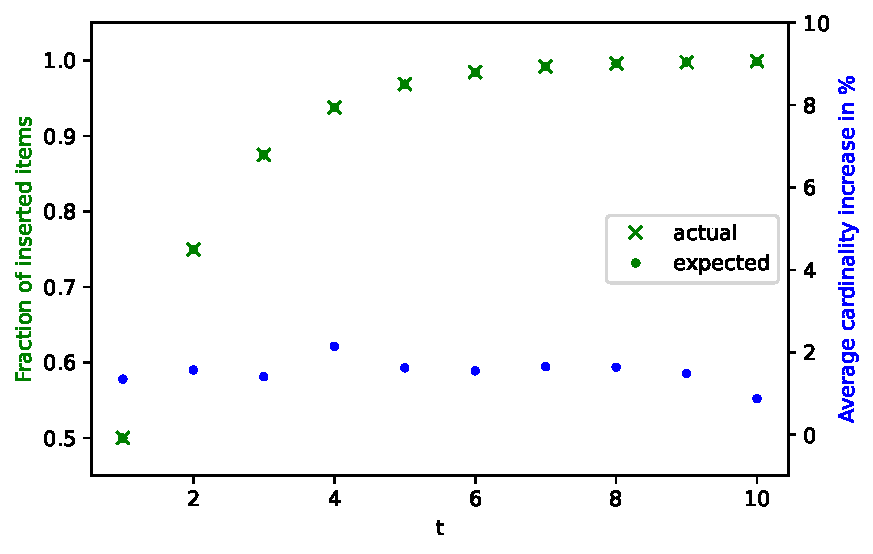
\includegraphics[width=0.9\textwidth]{figures/graph_S2.pdf}
    \end{minipage}\hfill
    \begin{minipage}{0.45\textwidth}
        \centering
        \caption{\DIFaddFL{Attack results as function of $t$ in scenario S4 with initially non-empty HLL sketch.}}\label{fig:graphS4}
        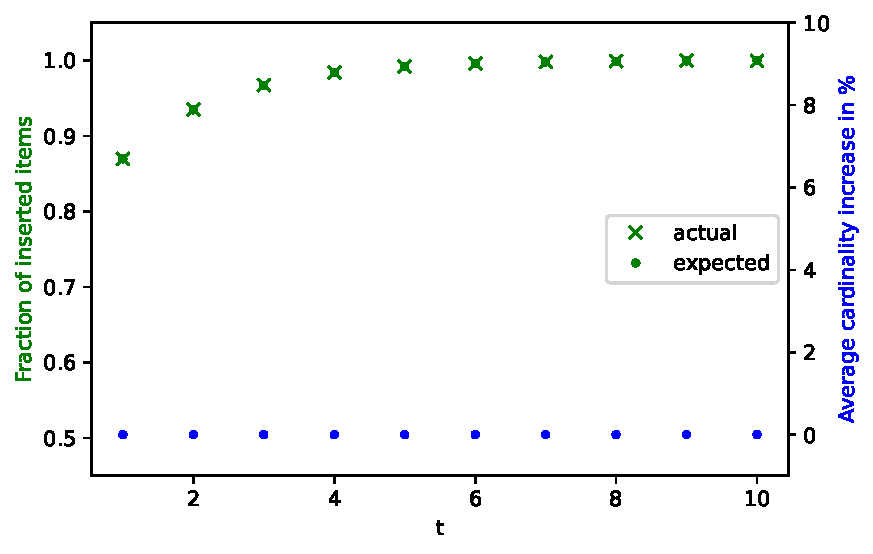
\includegraphics[width=0.9\textwidth]{figures/graph_S4.pdf} %DIF >  second figure itself
     \end{minipage}

     \begin{minipage}{0.45\textwidth}
        \centering
        \caption{\DIFaddFL{Attack results as function of $t$ for HLL in Redis (scenario S2) with initially non-empty HLL sketch.}}\label{fig:graphRedis}
        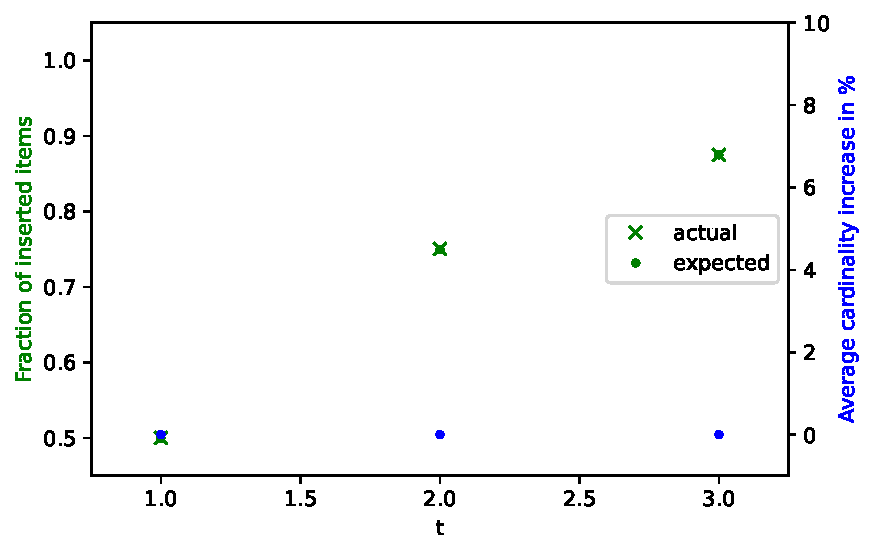
\includegraphics[width=0.9\textwidth]{figures/graph_redis.pdf} %DIF >  second figure itself
     \end{minipage}
\end{figure*}

%DIF > \begin{table*}[tb!]
%DIF > \small\centering
%DIF > \caption{Original Table: Attack results for a classic HLL implementation, averaged over 50 iterations, in the setting of~\cite{hllvuln}.}
%DIF > \medskip
%DIF >      \makebox[\linewidth]{
%DIF > \begin{tabular}{| m{11em} | m{3.4em} | m{4.8em} | m{4.1em} | m{4.1em} | m{4.1em} | m{4em} |}
%DIF >     \hline
%DIF >     \textbf{Scenario} & \multicolumn{2}{c|}{S1} & \multicolumn{2}{c|}{S2} & \multicolumn{2}{c|}{S4} \\ \hline
%DIF >     %\textbf{HLL initially empty?} & yes & yes & yes & no & yes & no \\ \hline
%DIF >       \textbf{Original Card. Est.} & 0 & 0 & 0 & 1,001 & 0 & 1,003 \\ \hline
%DIF >        \textbf{\# Targeted buckets $B$} & 1 & 128 (= m/2) & 1 & - & 1 & - \\ \hline
%DIF >      \textbf{\# Items added} & 977 & 125,091 & 980 & 125,153 & 1,003 & 204,127 \\ \hline
%DIF >     \textbf{Final Card. Est.} & 1 & 177 & 1 & 1,058  & 1 & 1,003 \\ \hline
%DIF >     \textbf{\# Resets} & 1,148 & 1,655 & - & - & - & - \\ \hline
%DIF > 
%DIF > \end{tabular}}
%DIF > \label{table:tab2bis}
%DIF > \end{table*}

\DIFaddend \subsection{Results for Redis}
We also implemented our attacks for the HLL implementation used in Redis as described in Section~\ref{sec:redis}.
The hash function $h$ is fixed as the 64-bit MurmurHash3 function. The seed used internally is hardcoded and can be extracted by inspection of the openly-available Redis codebase.
Furthermore, the number of buckets is constant and set to 16,384. Knowledge of these parameters places us in the setting of an S2 adversary.
Since a classic Redis application separates the server holding the sketch from the client interacting with the sketch, we consider that attack scenarios S3 or S4, while possible, are not typical for Redis. 
Thus, we only consider scenario S2 for Redis.
\DIFdelbegin \DIFdel{For simplicity, we }\DIFdelend \DIFaddbegin \DIFadd{We }\DIFaddend set attack parameter $\epsilon$ to $\frac{1}{2}$ \DIFaddbegin \DIFadd{and then $\frac{1}{4}$ }\DIFaddend in the attack on an initially empty HLL sketch. \DIFaddbegin \DIFadd{We recall that this will lead to the number of empty buckets $C_0$ to be equal to $\frac{m}{2} (=8,192)$ and $\frac{m}{4} (=4,096)$ respectively.
}\DIFaddend The results are averaged over \DIFdelbegin \DIFdel{30 }\DIFdelend \DIFaddbegin \DIFadd{50 }\DIFaddend iterations and reported in Table~\ref{table:tab3}. \DIFaddbegin \DIFadd{Meanwhile, Figure~\ref{fig:graphRedis} shows our results for an initially non-empty sketch as a function of $t$, where $2^{t-1}m\ln m$ items are honestly inserted into the sketch. }\DIFaddend Similarly to the case for classic HLL, our empirical results \DIFdelbegin \DIFdel{match }\DIFdelend \DIFaddbegin \DIFadd{in  Table~\ref{table:tab3} and Figure~\ref{fig:graphRedis} match closely }\DIFaddend with our theoretical \DIFdelbegin \DIFdel{analysis}\DIFdelend \DIFaddbegin \DIFadd{analyses}\DIFaddend .

\begin{table*}[tb!]
\DIFdelbeginFL %DIFDELCMD < \small\centering
%DIFDELCMD < %%%
\DIFdelendFL \DIFaddbeginFL \begin{center}
\DIFaddendFL \caption{Attack results \DIFaddbeginFL \DIFaddFL{on initially empty sketches }\DIFaddendFL for HLL in Redis \DIFaddbeginFL \DIFaddFL{(scenario S2)}\DIFaddendFL , \DIFaddbeginFL \\ \DIFaddendFL averaged over \DIFdelbeginFL \DIFdelFL{30 }\DIFdelendFL \DIFaddbeginFL \DIFaddFL{50 }\DIFaddendFL iterations.}\DIFdelbeginFL %DIFDELCMD < \medskip
%DIFDELCMD <      %%%
\DIFdelFL{\makebox[\linewidth]{
\begin{tabular}{| m{11em} | m{4em} | m{4.2em} |}
    \hline
    \textbf{Scenario} &  \multicolumn{2}{c|}{S2} \\ \hline
    \textbf{$\epsilon$} & n/a & 0.5 \\ \hline
    \textbf{HLL initially empty?} & no & yes \\ \hline
    \textbf{Original Card. Est.} & 70,140 & 0 \\ \hline
    \textbf{\# Items added} & 524,455 & 524,275 \\ \hline
    \textbf{Final Card. Est.} & 73,249 & 13,188 \\ \hline
\end{tabular}}
}\DIFdelendFL \label{table:tab3}
%DIF > \begin{tabular}{| m{11em} | m{4em} | m{4.2em} |}
\DIFaddbeginFL \begin{tabular}{| l | r | r |}
    \hline
    \textbf{\DIFaddFL{Original Card. Est.}} & \DIFaddFL{0 }& \DIFaddFL{0 }\\ \hline
     \textbf{\DIFaddFL{$\epsilon$}} &  \DIFaddFL{0.5 }& \DIFaddFL{0.25  }\\ \hline
    \textbf{\DIFaddFL{\# Items added}} &  \DIFaddFL{524,2104 }& \DIFaddFL{785,920 }\\ \hline
    \textbf{\DIFaddFL{Final Card. Est.}} & \DIFaddFL{13,185 }& \DIFaddFL{35,938}\\ \hline
\end{tabular}
\end{center}
\DIFaddendFL \end{table*}
%\todo[inline]{Results from Redis or GBQ if we get them.}

%DIF >     \textbf{Original Card. Est.} & 0 & 139,967 \\ \hline
%DIF >      \textbf{$\epsilon$} &  0.5 & - \\ \hline
%DIF >     \textbf{\# Items added} & 524,210 & 524,454\\ \hline
%DIF >     \textbf{Final Card. Est.} & 13,185 & 139,967 \\ \hline
\DIFaddbegin 

\DIFaddend \subsection{Relating the Attacks to Applications}\label{sec:exp-apps}

So far, we have treated attacks in an abstract way, working with an off-the-shelf implementation of HLL. We now illustrate what effect such attacks might have on applications relying on HLL for cardinality estimation. Specifically, we analyse a recent paper~\cite{flexswitch} from the networking systems community.

The authors of~\cite{flexswitch} propose to use HLL for recording traffic flow statistics in datacenter network switches. The idea is to use HLL so as to reduce the amount of memory needed in the switches. The resulting switches are called \emph{flexswitches} in~\cite{flexswitch}. In the main example considered in~\cite[Section 3.1]{flexswitch}, each flow is identified by a 4-tuple consisting of source IP address, destination IP address, source port, and destination port. Various parameters for the HLL sketch to be used are then explored in~\cite{flexswitch}, trading memory consumed for accuracy of estimation of the number of concurrent flows. The paper also proposes to use the low range correction method of Fig.~\ref{fig:hll}. At no point does the discussion in~\cite{flexswitch} consider adversarial input (it does mention worst-case performance but only in passing, and no indication is given of how to handle this). It is clear that, by modifying the 16-bit source port (for example), an adversary could fool the switch into undercounting the flows the adversary is responsible for producing. Depending on how the flow count is used, this could lead to undetected DoS conditions, mis-provisioning of network capacity, or under-billing of the adversary for its traffic. In Appendix~\ref{sec:flexswitch} we provide further analysis showing that each use of HLL proposed in~\cite{flexswitch} can be subverted by an S2 adversary.

%\todo[inline]{This ends up being pretty harsh on this NSDI paper, but hey. We may shorten or move some details to an appendix.}

\section{Formal Security Analysis}\label{sec:formal}

In this section we present a formal security analysis of HLL, focussing on how to augment the original HLL design with cryptographic mechanisms and thereby provably prevent attacks. We focus on the case of an initially empty HLL sketch, giving the adversary full control over which items are inserted into it.

\subsection{Scenario S1}
We begin by disposing of scenario S1. In that scenario, the attacker has access to insertion and reset capabilities, and to cardinality estimates, for a shadow HLL that is identical in every respect to the target HLL. The attacks we presented previously are oblivious to any internals of the implementation (other than that they follow the HLL description in Figure~\ref{fig:hll}). This means that, say, replacing the hash function $h$ with a keyed function or any other cryptographic primitive would be futile in preventing attacks in scenario S1. Interestingly, our attacks in scenario S1 are more complex and require more effort than in scenarios S2 and S4. The fact that we cannot prove security in S1 with improved cryptography is not in contradiction to this, but rather an illustration of the power conferred by giving the adversary access to an exact and resettable replica of the target device in the keyed setting.

In summary, we cannot hope to gain any security in scenario S1 by adding more cryptography.

\subsection{Intuition for Formal Security Analysis}\label{sec:informal}

For scenarios S2, S3 and S4, the picture is much more positive. In the remainder of this section, we introduce a formal security model covering all three scenarios. We work with a simulation-based framework, in contrast to the game-based approach introduced for probabilistic data structures in~\cite{CCS:ClaPatShrPS19}. %We discuss the strengths of our alternative approach in more detail below. 

We first begin by explaining the high-level idea of our approach. We allow an adversary ${\mathcal{A}}$ to interact with an HLL sketch via various oracles that capture its capabilities in each of the three scenarios S2, S3 and S4: it may have an \texttt{insert($\cdot$)} oracle allowing it to add items to the HLL sketch, a \texttt{read} oracle that returns the HLL cardinality estimate, and a \texttt{corrupt} that returns all the HLL sketch's bucket contents (but not any secret key $K$); in S4 it has all three oracles. In addition, in all 3 scenarios, ${\mathcal{A}}$ has access to an \texttt{init($\cdot$)} oracle by which it sets the HLL parameters $n$, $m=2^n$, $\ell$, $\alpha_m$ used to initialise the HLL sketch. We assume ${\mathcal{A}}$ always makes exactly one \texttt{init($\cdot$)} query and that it is its first oracle call.

In the security model, the game selects at random one of two worlds by sampling a bit $b$. In the real world ($b=0$), ${\mathcal{A}}$ interacts with the scheme HLL-$F$. This is the same as HLL operating as in Figure~\ref{fig:hll} but where the hash function $h$ is replaced by a keyed function $F: \{0,1\}^k \times {{\hat{\mathcal{D}}}} \rightarrow  \{0,1\}^{n+\ell}$ whose key $K$ is sampled uniformly at random at the beginning of the game and not available to the adversary; ${\mathcal{A}}$ has access to the relevant selection of oracles and completes its execution with some output $\textsf{out}_{\mathcal{A}}$ (a bit-string).

In the ideal world ($b=1$), ${\mathcal{A}}$ is replaced by a simulator ${\mathcal{S}}$ with blackbox oracle access to ${\mathcal{A}}$ (that is, ${\mathcal{S}}$ can run ${\mathcal{A}}$ in a blackbox manner, receiving its oracle queries and providing responses to ${\mathcal{A}}$ as it sees fit). In particular, ${\mathcal{S}}$ receives parameters $n$, $\ell$, $\alpha_m$ from ${\mathcal{A}}$'s \texttt{init($\cdot$)} call. Finally, ${\mathcal{S}}$ receives $\textsf{out}_{\mathcal{A}}$ and completes its execution by producing its own output $\textsf{out}_{\mathcal{S}}$. 

Importantly, we will specify an ${\mathcal{S}}$ that handles all of ${\mathcal{A}}$'s \texttt{insert($x$)} queries using \emph{random sampling}, that is, by setting $y \leftarrow_{\$} \{0,1\}^{n+\ell}$ instead of $y: = F_K(x)$ and then executing the rest of the insertion process as in Figure~\ref{fig:hll}. In essence, our ${\mathcal{S}}$ will build its own ``shadow'' HLL in which all insertion queries are handled by random sampling. ${\mathcal{S}}$ then uses the shadow HLL for handling ${\mathcal{A}}$'s \texttt{read} and \texttt{corrupt} queries. Finally, we will specify ${\mathcal{S}}$ so that it outputs whatever ${\mathcal{A}}$ outputs.

We will prove that  ${\mathcal{S}}$ is such that, given any adversary ${\mathcal{A}}$, then any distinguisher $\mathcal{D}$ that can distinguish between the $\textsf{out}_{\mathcal{A}}$ in the real world and $\textsf{out}_{\mathcal{S}}$ in the ideal world can be used to build an adversary ${{\mathcal{B}}}$ which breaks the PRF security of $F$. Under the assumption that $F$ is a good PRF, no such efficient distinguisher $\mathcal{D}$ can exist, and we may conclude that (up to PRF security) no efficient distinguisher can tell that it is interacting with the ideal world instead of the real world. 

Why does this proof imply that ${\mathcal{A}}$ cannot manipulate the cardinality estimate? To see this, note that (amongst many other possibilities) ${\mathcal{A}}$'s output could be the cardinality estimate obtained from a \texttt{read} query, allowing a specific ${\mathcal{D}}$ to try to use that to distinguish between the two worlds. Yet, by the preceding argument, the simulator in the ideal world is able to produce an output that ${\mathcal{D}}$ cannot distinguish from that of ${\mathcal{A}}$ in the real world. In particular, our simulator will output whatever ${\mathcal{A}}$ outputs, so if ${\mathcal{A}}$'s output $\textsf{out}_{\mathcal{A}}$ is the result of a \texttt{read} query in the ideal world, then so will ${\mathcal{S}}$'s. But in the ideal world, ${\mathcal{S}}$ uses random sampling for the $y$ values, so in that world ${\mathcal{S}}$ (and ${\mathcal{A}}$ that it runs) are operating in the setting where the average case analysis of HLL applies, as per~\cite{hll}. So in the ideal world this specific ${\mathcal{D}}$ would receive an accurate average case cardinality estimate. Since ${\mathcal{D}}$ tries to distinguish the two worlds from the cardinality estimate and we already showed that no efficient distinguisher ${{\mathcal{D}}}$ can exist, it must follow that the cardinality estimates produced in the real and ideal worlds are indistinguishable (up to PRF security). It then follows that ${\mathcal{A}}$ has no advantage when it comes to manipulating the HLL-$F$ cardinality estimate. So HLL, when instantiated with PRF $F$, is secure against cardinality manipulation attacks.
% in S4 (and therefore in the weaker attacks models S2 and S3 as well). 

%We will conclude our analysis by discussing how $F$ can be instantiated.

\subsection{Formal Security Model for HLL}

We now formalise the above intuition. Our definitions are specific to HLL-$F$ as the object of analysis, but are easily generalised to any cardinality estimator with the same syntax as HLL-$F$ (that can be formally defined by a triple of algorithms (\texttt{Init}, \texttt{Insert}, \texttt{Read})).

\vspace{0.2cm}
\noindent\textbf{The distinguisher ${\mathcal{D}}$ and its advantage.} We consider distinguisher ${\mathcal{D}}$ to be an algorithm running in a security game. The game begins with the selection of a bit $b$ uniformly at random and then runs either adversary ${\mathcal{A}}$ (the real world, $b=0$) or simulator ${\mathcal{S}}$ (the ideal world, $b=1$). Adversary ${\mathcal{A}}$ interacts with up to four oracles which are handled by the game using the algorithms of HLL-$F$. These are defined below; different combinations of oracles define scenarios S2, S3, S4. After making some queries, ${\mathcal{A}}$ returns its output $\textsf{out}_{\mathcal{A}}$ to ${\mathcal{D}}$. Simulator ${\mathcal{S}}$ runs ${\mathcal{A}}$ in a blackbox manner (as specified below) and receives ${\mathcal{A}}$'s output. It then provides its own output $\textsf{out}_{\mathcal{S}}$ to ${\mathcal{D}}$. Finally, ${\mathcal{D}}$ outputs a bit $b'$ estimating whether it is interacting with the real world ($b'=0$) or the ideal world ($b'=1$). For $i=2, 3, 4$, we define ${\mathcal{D}}$'s S$i$-Real-or-Ideal advantage against HLL-$F$ with adversary ${\mathcal{A}}$ and simulator ${\mathcal{S}}$ to be:
\[
\mbox{Adv}^{\mbox{\tiny S$i$-RoI}}_{\mbox{\tiny{HLL-$F$,${\mathcal{A}}$,${\mathcal{S}}$}}}({\mathcal{D}}) := \lvert 2\Pr[b' = b] - 1 \rvert \, .
\]
%Using a standard transformation, this probability can be rewritten as $\lvert \Pr[b' = 1| b = 1] - \Pr[b'=0|b=1] \rvert$. 

\vspace{0.2cm}
\noindent\textbf{The adversary ${\mathcal{A}}$ and its oracles.}
The four oracles that  ${\mathcal{A}}$ can interact with behave as follows in the real world:
\begin{itemize}
\item \texttt{init($\cdot$)}: this oracle receives as input the HLL-$F$ parameters ($n$, $\ell$, $\alpha_m$) and performs initialisation of the HLL-$F$ sketch, including generating the array of $m=2^n$ buckets $M[j]$ and initialising all the entries to $0$, and selecting a key $K \leftarrow_{\$} \{0,1\}^k$ for keyed function $F: \{0,1\}^k \times {{\hat{\mathcal{D}}}} \rightarrow  \{0,1\}^{n+\ell}$. This oracle has no output. It is available in all of S2, S3, S4. We assume it is only called once as ${\mathcal{A}}$'s first oracle query.
\item \texttt{insert($\cdot$)}: on input $x \in {{\hat{\mathcal{D}}}}$, the oracle implements HLL-$F$ by setting $y = F_K(x)$ and following the procedure in Figure~\ref{fig:hll} to insert $x$ into the HLL sketch (that is, it uses the first $n$ bits of $y$ to determine a bucket index $j$ and the next $\ell$ bits of $y$ to determine a bit-string $w$; then $\rho(w)$ is used to update the bucket at index $j$ via $M[j]:= \max(M[j],\rho(w))$). This oracle has no output. It is available in all of S2, S3, S4. Since HLL and variants of it we consider here have the property that reinserting an item $x$ does not change the internal state of the HLL sketch (nor the cardinality estimate computed from it) we assume without loss of generality that all queries $x$ made by ${\mathcal{A}}$ to \texttt{insert($\cdot$)} are distinct.
\item \texttt{read}: this oracle has no input and returns the HLL-$F$ cardinality estimate as per Figure~\ref{fig:hll}, i.e.\ it computes a raw cardinality estimate via $E := \alpha_mm^2\cdot(\sum_{j=1}^m2^{-M[j]})^{-1}$ and then performs corrections for small and large values. We allow multiple queries to this oracle and make it available to ${\mathcal{A}}$ in S3 and S4, but not S2.
\item \texttt{corrupt}: this oracle has no input and returns the vector $(M[j])_{j=1}^{m}$ of HLL bucket contents (but not any secret key $K$). This oracle is available only in S4. We allow the adversary to query \texttt{corrupt} as often as it wishes during its attack. Our description of S4 in Section~\ref{sec:attacks} limited the adversary to at most one such query; here we allow multiple queries because doing so does not increase the difficulty of achieving security.  
\end{itemize}

We note that in S4 (and only in S4) the adversary has access to all four oracles. This makes it the strongest model, and hereafter we only target security in this model. 

\vspace{0.2cm}
\noindent\textbf{A specific simulator ${\mathcal{S}}$.} In order to obtain a meaningful security definition that prevents cardinality manipulation, we need to restrict ${\mathcal{S}}$ to doing random sampling when handling \texttt{insert($\cdot$)} queries coming from ${\mathcal{A}}$. Otherwise, our definition could be vacuously satisfied (for example ${\mathcal{S}}$ could just sample the PRF key $K$ for itself and provide a perfect real-world view). This is somewhat different to typical simulation-based security definitions, where ${\mathcal{S}}$'s behaviour is not restricted but its input might be (e.g.\ in a confidentiality definition, ${\mathcal{S}}$ might receive only $|m|$ in place of plaintext $m$). Crucially, in our setting, security arises from inspecting the details of ${\mathcal{S}}$ and observing that, due to its use of random sampling, it instantiates HLL in the average case.

In full detail, our specific ${\mathcal{S}}$ operates by running ${\mathcal{A}}$ in a blackbox manner and handling all of its queries as follows:
\begin{itemize}
\item \texttt{init($\cdot$)}: on input $n$, $\ell$, $\alpha_m$, ${\mathcal{S}}$ initialises an HLL sketch as in Figure~\ref{fig:hll}; that is, it creates an array of $m=2^n$ buckets $M[j]$ and initialises them all to 0.
\item \texttt{insert($\cdot$)}: on input $x \in {{\hat{\mathcal{D}}}}$,  ${\mathcal{S}}$ ignores $x$, sets $y \leftarrow_{\$} \{0,1\}^{n+\ell}$, and proceeds to update the buckets using this value of $y$ as in the original HLL algorithm in Figure~\ref{fig:hll}.
\item \texttt{read}:  ${\mathcal{S}}$ returns the HLL cardinality estimate computed as per Figure~\ref{fig:hll}.
\item \texttt{corrupt}: ${\mathcal{S}}$ returns the current vector $(M[j])_{j=1}^{m}$ of HLL bucket contents that it has stored.
\end{itemize}
At the end of ${\mathcal{A}}$'s execution, ${\mathcal{S}}$ takes ${\mathcal{A}}$'s output $\textsf{out}_{\mathcal{A}}$ and forwards it to ${\mathcal{D}}$ as its own output $\textsf{out}_{\mathcal{S}}$. Notice that the running time $t_{\mathcal{S}}$ of ${\mathcal{S}}$ is (roughly) equal to that of ${\mathcal{A}}$.

\vspace{0.2cm}
\noindent\textbf{Formal security definition and main result.} Now we are ready to give:
\begin{definition}
The scheme HLL-$F$ is S$i$-simulation-secure with parameters $(q,t_{\mathcal{S}},t_{\mathcal{A}},t_{\mathcal{D}},\epsilon)$ if, for the specific simulator $\mathcal{S}$ given above, for all adversaries ${\mathcal{A}}$ running in time at most $t_{\mathcal{A}}$ and making at most $q$ \texttt{insert($\cdot$)} queries, and for all distinguishers ${\mathcal{D}}$ running in time at most $t_{\mathcal{D}}$, we have
$\mbox{Adv}^{\mbox{\tiny S$i$-RoI}}_{\mbox{\tiny{HLL-$F$,${\mathcal{A}}$,${\mathcal{S}}$}}}({\mathcal{D}}) \leq \epsilon$. 
\end{definition}

In the above definition, we quantify over \texttt{insert($\cdot$)} queries (via $q$) and not other types of query because only \texttt{insert($\cdot$)} queries will appear in our concrete security analysis and we do not want to clutter the notation. Note also that our definition is given with respect to a \emph{specific} simulator, but could be generalised to allow any simulator that performs random sampling when handling \texttt{insert($\cdot$)} queries.

Our simulation-based security definition does not require us to specify a winning condition for adversary $\mathcal{A}$. Rather, we infer from inspecting the simulator what the adversary can (or cannot) achieve in the ideal world, and show that no efficient algorithm $\mathcal{D}$ can distinguish the real and ideal worlds. This is in contrast to the game-based approach of~\cite{CCS:ClaPatShrPS19} which needs a complex definition to say when the adversary has successfully manipulated a probabilistic data structure. This reveals a strength of the simulation-based approach.


Before stating our main result, we require one further standard definition:
\begin{definition}
Let $F: \{0,1\}^k \times {{\hat{\mathcal{D}}}} \rightarrow  \{0,1\}^{n+\ell}$.
We define the PRF advantage of an adversary ${{\mathcal{B}}}$ against $F$ outputting a bit $d'$ as being its advantage in distinguishing whether it is interacting with $F$ for a uniformly random key $K$ ($d=0$) or interacting with a truly random function ($d=1$). We write: 
\[
\mbox{Adv}^{\mbox{\tiny PRF}}_{F}({{\mathcal{B}}}) := \lvert 2\Pr[d' = d] - 1 \rvert\,.
\]
\end{definition}
Here, we assume without loss of generality that all of ${{\mathcal{B}}}$'s queries are distinct. See~\cite[Section 4.4.1]{BonehShoup} for details of the PRF security definition.


Now we are ready to formally state our main result. The proof can be found in Appendix~\ref{sec:proof}.
\begin{theorem}\label{thm:security-of-HLL-with-PRF}
Let simulator $\mathcal{S}$ be as described above. For any S4 adversary ${\mathcal{A}}$ against HLL-$F$ and any distinguisher $\mathcal{D}$, we can construct a PRF adversary ${{\mathcal{B}}}$ against $F$ such that:
\[
 \mbox{Adv}^{\mbox{\tiny PRF}}_{F}({{\mathcal{B}}}) = 
 \mbox{Adv}^{\mbox{\tiny S$4$-RoI}}_{\mbox{\tiny{HLL-$F$,${\mathcal{A}}$,${\mathcal{S}}$}}}({\mathcal{D}}) \,.
\]
Moreover, if ${\mathcal{A}}$ makes $q$ queries to its \texttt{insert($\cdot$)} oracle, then ${{\mathcal{B}}}$ makes $q$ queries to its real or random oracle. Finally, the running time of ${{\mathcal{B}}}$ is (roughly) $t_{\mathcal{A}}+t_{\mathcal{D}}$.
\end{theorem}

This result tightly relates the security of HLL-$F$ against cardinality manipulation to that of the PRF security of the function $F$ used in its construction (for the reasons explained in Section~\ref{sec:informal}).

%Informally, if $F$ is a good PRF, then $\mbox{Adv}^{\mbox{\tiny PRF}}_{F}({{\mathcal{B}}})$ should be small for any adversary ${{\mathcal{B}}}$ running in a reasonable amount of time; hence the advantage of any S4 adversary  ${\mathcal{A}}$ against HLL using PRF $F$ is also small. 
%Note that our proof would still apply for the algorithm of~\cite{hllnew} that is used in Redis if it used a PRF in place of a hash function. The only change needed is to use the Redis approach for computing responses to \texttt{read} queries in place of the classical HLL approach.


\subsection{On Confidentiality}

An HLL sketch can leak information about items $x$ that were previously inserted. Consider the following attack from~\cite{cardestprivacy}: to test whether an item $x$ was previously inserted into the HLL by an honest user (say), the adversary makes a sequence of queries: \texttt{read}, \texttt{insert($x$)}, \texttt{read}. If the two cardinality estimates are different, the adversary can conclude definitively that $x$ was \emph{not} previously inserted into the HLL; if they are the same, it can estimate (with some error) that $x$ was previously inserted.\footnote{Errors can arise in two ways when $x$ was not previously inserted: either inserting $x$ changes a bucket value, but the change is masked by rounding when the cardinality estimate is computed, or inserting $x$ does lead to a change in a bucket value because $\rho(w)$ computed from $x$ is too small.} This attack still works even if HLL is implemented using a PRF and is unavoidable in view of the oracle queries (and in real settings, the API) available to the adversary. So such privacy leaks are an inherent feature of HLL if a rich enough API is provided. Note that this attack does not contradict our main result, which concerns prevention of cardinality manipulation rather than confidentiality. 

%\todo[inline]{
%Still, simulation-based security notions are often used to model confidentiality properties, so it is tempting to think that our security definition might say something about confidentiality of the HLL inputs $x$. Our existing model does not, since ${\mathcal{A}}$ chooses all the inputs $x$ and so ``knows'' them already. However, it is easily modified to provide a confidentiality notion. For example, we can consider the insertion of honestly generated items $x$ that are drawn from some probability distribution $p$ on $\hat{\mathcal{D}}$ in a first phase, with ${\mathcal{A}}$ then having access to only \texttt{read} and \texttt{corrupt} oracles in a second phase (we have to remove the \texttt{insert($\cdot$)} oracle in view of the general attack from~\cite{cardestprivacy}). 

%In this case, the simulator ${\mathcal{S}}$ in the ideal world can proceed without ever seeing any inputs but instead knowing only the distribution $p$ and the number of distinct samples drawn from it in the first phase. It is not hard to modify the proof of Theorem~\ref{thm:security-of-HLL-with-PRF} to show that no adversary can distinguish real and ideal worlds in this case (up to PRF security). Now, since ${\mathcal{S}}$ has no access to inputs $x$, we can conclude that the HLL implemented using a PRF ensures confidentiality for the inputs $x$. Thus, the cardinality estimates and even the bucket values themselves do not leak information about the honestly inserted values $x$ (beyond their number). }

We leave the exploration of the adaptation of our simulation-based security definitions to capture confidentiality notions for more restricted APIs to future work. 

\subsection{Is Universal Hashing Sufficient?}

It is natural to wonder whether a PRF is really required in place of hash function $h$ in order to make HLL secure, or whether a weaker cryptographic primitive would suffice. For example, since it has (roughly) uniform outputs, perhaps using a universal hash function (UHF) $h_K(\cdot)$ would be sufficient. In Appendix~\ref{sec:UHF} we \DIFdelbegin \DIFdel{show that, in general, UHFs do not suffice by providing }\DIFdelend \DIFaddbegin \DIFadd{provide }\DIFaddend a key recovery attack against HLL when $h$ is replaced by a \DIFdelbegin \DIFdel{specific }\DIFdelend \DIFaddbegin \emph{\DIFadd{specific}} \DIFaddend UHF based on polynomial evaluation over a finite field. \DIFaddbegin \DIFadd{This is enough to show that UHFs do not suffice in general. 
}\DIFaddend 

\subsection{Instantiating the PRF}

Our HLL construction requires a PRF $F: \{0,1\}^k \times {{\hat{\mathcal{D}}}} \rightarrow  \{0,1\}^{n+\ell}$. Here, the set ${{\hat{\mathcal{D}}}}$ represents the space of possible inputs to HLL which can be modelled by a set of bit-strings of some maximum length. This means that $F$ needs to be Variable Input Length PRF (VIL-PRF). 

\DIFdelbegin \DIFdel{We }\DIFdelend \DIFaddbegin \DIFadd{From inspection of Figure~\ref{fig:hll}, it is evident that hashing is the dominant cost when inserting an item into HLL. So we }\DIFaddend want $F$ to be competitive with non-cryptographic hashing\DIFaddbegin \DIFadd{, especially }\DIFaddend on small input sizes \DIFdelbegin \DIFdel{, }\DIFdelend \DIFaddbegin \DIFadd{(}\DIFaddend as typical in current HLL implementations and applications\DIFdelbegin \DIFdel{(}\DIFdelend \DIFaddbegin \DIFadd{, }\DIFaddend e.g.\ MurmurHash3 applied to an IP header). This makes off-the-shelf approaches like HMAC uncompetitive, since even for the shortest inputs, HMAC would require 4 evaluations of the underlying hash compression function.

SipHash~\cite{AumassonB12} is designed specifically for this use case. It is competitive in speed with non-cryptographic hash functions commonly used in HLL implementations such as MurmurHash3. It has also withstood cryptanalysis well~\cite{DobraunigMS14,XinLSL19}. It has 128-bit outputs that can be truncated to the needs of typical HLL implementations (32 and 64 bits). %and is well supported in libraries such as OpenSSL.  
Our microbenchmarks created on an Intel i7 CPU show that SipHash-2-4 on 90-byte inputs requires 102ns per evaluation, while the 128-bit version of MurmurHash3 takes 60ns. Meanwhile, HMAC-SHA256 requires 705ns. We obtained similar performance ratios for other input sizes. These together show that SipHash is quite competitive with MurmurHash3. 

%is as fast as the 128-bit version of MurmurHash3 and only slightly slower than the original 32-bit version.

%length: 720, time h_mac 705ns, time h_murmur 60ns and time h_sip 102ns


%Making $F$ competitive in speed with existing implementations of HLL, which use non-cryptographic hash functions such as Murmur3, is challenging, and in practice we must sacrifice some speed for security.

%A particularly simple construction for $F$ involves composing a collision-resistant hash function $H: {{\hat{\mathcal{D}}}} \rightarrow  {\cal E}$ onto some domain ${\cal E}$ with a PRF $G: \{0,1\}^k \times {\cal E} \rightarrow \{0,1\}^{n+\ell}$, viz: $F(K,x) = G(K,H(x))$. The result is a PRF with the required input-output signature~\cite[Section 8.2]{BonehShoup}. As a concrete instantiation, one could take $H$ to be SHA-256 with outputs truncated to 128 bits and $G$ to be AES-128 truncated to ${n+\ell}$ bits (since ${n+\ell} \leq 64 < 128$ in practice, this truncation is always possible). 

%An alternative is to simply use HMAC-SHA-256 with an appropriately truncated output. HMAC is a PRF under reasonable assumptions on the hash function used in its construction~\cite{Bellare15}. 

%These constructions would be relatively fast on commodity platforms due to widespread hardware support for SHA-256 and AES operations. It would be a simple exercise to add the above PRF proposals to an existing HLL implementation and benchmark them against, say, Murmur3.  The exact slowdown depends on platform specifics, but based on microbenchmarks can be expected to be in the range 2-fold to 5-fold compared to Murmur3. \todo{Put a hard number here.}

%More complex but faster constructions using randomised or nonce-based MACs constructed from universal hashing could be envisaged. However, these do not seem to be directly applicable here since we need the function $F$ to be both stateless and deterministic so as to cope with the repeated inputs one would encounter during the normal operation of HLL.

We note that using keyed functions sacrifices the mergeability property that HLL enjoys, if different keys $K$ are used in different HLL sketches. The reason is that one can no longer emulate running a single HLL sketch by taking the maximum over all buckets with each index $j$ in the different sketches, since now the bucket contents are created using different keys in a PRF and hence bear no relation to one another. 

%\todo{Discussion: note again that no-one currently does this in practice; also point out that you want different keys in different sketches for security, but this sacrifices the merge capability of HLL.}


\section{Conclusion}\label{sec:conclusions}
The HyperLogLog algorithm is an elegant and efficient solution to the problem of estimating the cardinality of large sets. Its simple structure makes it easy to code and use, as shown by the growing number of available open-source implementations. Nonetheless, we have shown that malicious users can manipulate the HLL cardinality estimate and thence break the security properties of systems relying on HLL. Our attacks are simple but powerful and should raise awareness of the limitations of HLL. Our analysis may assist software developers in understanding the risks they run when using HLL in adversarial settings. We have also provided a method for securing HLL in adversarial settings: simply replace the internal hash function by a keyed PRF, and one obtains full protection even in scenario S4, our strongest attack scenario. %However, this solution requires the introduction of a cryptographic key, and all the attendant key management issues this brings. So while the solution is simple on paper, in practice, it is less so. 

%Future work could consist in finding mitigations that do not rely on salt. For example, would the imposed ID setting (like Facebook) solve the issue but still be convenient for the various HLL applications?
Left to future work is the task of extending our attacks and defences to HLL variants such as sliding HLL~\cite{slidinghll} and HLL++~\cite{hllpractice}. It would be interesting to find and analyse a strategy for more cleverly ordering the candidates in our attack in scenario S1 to reduce the total insertion cost of the attack, whilst also keeping the number of resets low. Finding an attack in scenario S1 when the target HLL sketch is initially non-empty is also open.

We have given a formal analysis of using a PRF as a countermeasure to our attacks. The use of a keyed function sacrifices HLL mergeability when the keys in the different HLLs are independently generated. It is an open problem to find methods for securing HLL sketches against adversarial inputs whilst retaining some form of mergeability. This may also require the introduction of entirely new data structures that trade increased storage for mergeability and improved security. \DIFaddbegin \DIFadd{It is also an open problem to extend our simulation-based approach to formal analysis to other data structures.
}\DIFaddend 

%\todo{Sim based of indepednent interest, arguably more powerful than game-based notions with fixed winning predicates.}
%It is also an open problem to close the performance gap that exists between fast but non-cryptographic hashes used in HLL implementations today and the slower but cryptographically strong VIL-PRF that is needed to obtain security.

\ifanon
\else
\section*{Acknowledgements}
The work of Paterson is supported in part by a gift from VMware.

The authors thank Dennis Hofheinz and Anupama Unnikrishnan for useful discussions on simulation-based definitions, Tom Shrimpton for suggesting to look at GoogleBigQuery, \DIFdelbegin \DIFdel{and }\DIFdelend Eylon Yogev for drawing our attention to related work on streaming algorithms with adversarial inputs\DIFaddbegin \DIFadd{, and Angelika Steger for help with balls-into-bins arguments}\DIFaddend .
\fi

\bibliographystyle{ieeetr}
\DIFdelbegin %DIFDELCMD < \bibliography{ref.bib}
%DIFDELCMD < %%%
\DIFdelend \DIFaddbegin \bibliography{./ref.bib}
\DIFaddend 

\DIFdelbegin %DIFDELCMD < \appendix
%DIFDELCMD < %%%
\DIFdelend \DIFaddbegin \appendices
\DIFaddend 

\section{\DIFaddbegin \DIFadd{Further analysis of Flexswitches}}\label{sec:flexswitch}

Extending our analysis of~\cite{flexswitch} from the main body, \cite[Section 4.2]{flexswitch} proposes using HLL for detecting TCP port scans by counting observed destination port numbers in TCP packets with set SYN flags and reporting a scan event if the estimate exceeds a
set threshold. Using our attack techniques (specifically, in scenario S2), an attacker could complete a partial port scan of roughly half of all $2^{16}$ ports whilst keeping the HLL estimate below $0.693m$ where $m$ is the number of buckets used in HLL. While~\cite{flexswitch} is not specific about the value of $m$ actually used, the authors' focus on reducing memory usage indicates that $m$ would not be larger than $1024$.\footnote{The paper mentions using 1 byte counters in the buckets and states that using more than 1KB of memory ``only improves average error rates marginally''; we infer a maximum value of $m=1024$ from this.} It is not stated in~\cite{flexswitch} what threshold needs to be crossed to trigger an alarm, but we consider it plausible that it would be above $0.693 \cdot 1024 = 710$. 

Similarly,~\cite[Section 4.2]{flexswitch} proposes using HLL for detecting NTP amplification attacks by counting distinct source IP addresses arriving on UDP port 123 over a small time window. No further details are given, but it is clear that an S2 attacker with even limited flexibility in spoofing source IP addresses (e.g.\ within a private range used in the datacenter) could easily evade detection whilst delivering a large number of NTP requests, thus re-enabling the original attack.

In a more advanced application,~\cite[Section 4.3]{flexswitch} proposes to use HLL as a component in a novel, low-memory version of the RCP congestion control algorithm called RCP-Approx. Again HLL is used for estimating numbers of traffic flows. Obviously, our attack techniques could be used (in scenario S2) to cause RCP-Approx to underestimate the number of traffic flows, leading to non-detection of congestion and so enabling DoS attacks to go undetected. 

Similar remarks apply to the treatment of CONGA in~\cite[Section 4.5]{flexswitch}. CONGA is a congestion-aware load balancing system that splits TCP flows into flowlets (collections of IP packets) and allocates them to paths based on congestion feedback from remote switches. In the enhancements to CONGA proposed in~\cite{flexswitch}, HLL is used in the ``flow statistics'' building block for estimating flowlet statistics in switches; these estimates are sent back to a monitoring system and used to determine the load balancing configuration. This overall system can be abused by an S2 adversary, to cause flowlet numbers to be underestimated (or overestimated) and the load balancing to perform sub-optimally. For example, an adversary could cause all the switches to \emph{over}-estimate the number of flowlets they are handling and ask the load balancing system to send less traffic through them. This could result in a degradation in the total amount of traffic the load balancing system can handle (depending on what fail-safe mode it has). Or an attacker could cause all the switches to \emph{under}-estimate the number of flowlets they are handling, causing undetected congestion in the switches.

\section{\DIFaddbegin \DIFadd{Proof of Theorem 8.1}}\label{sec:proof} %ridiculous, but had to hard-code this reference

PRF adversary ${{\mathcal{B}}}$ against $F$ is built as follows. Let $d$ denote the hidden bit determining whether ${{\mathcal{B}}}$ receives real responses of the form $F_K(x)$ where $K$ is a uniformly random key ($d=0$) or responses from a truly random function ($d=1$); ${{\mathcal{B}}}$ provides a simulation of either the real or ideal world for distinguisher ${\mathcal{D}}$ as follows. ${{\mathcal{B}}}$ runs ${{\mathcal{A}}}$ and answers each of ${{\mathcal{A}}}$'s queries as follows:
\begin{itemize}
\item \texttt{init($\cdot$)}: ${{\mathcal{B}}}$ receives parameters $n$, $\ell$, $\alpha_m$, sets $m=2^n$ and initialises an array $M[j]$ of size $m$ in which each of the entries is set to 0. 
\item \texttt{insert($\cdot$)}: on input $x \in {{\hat{\mathcal{D}}}}$,  ${{\mathcal{B}}}$ makes a query on $x$ to its real-or-random oracle and receives value $y$; ${{\mathcal{B}}}$ uses $y$ to update the HLL sketch as in the regular HLL algorithm (shown in Figure~\ref{fig:hll}). That is, it uses the first $n$ bits of $y$ to determine a bucket index $j$ and the next $\ell$ bits of $y$ to determine a bit-string $w$; then $\rho(w)$ is used to update the bucket at index $j$ via $M[j]:= \max(M[j],\rho(w))$.
\item \texttt{read}: ${{\mathcal{B}}}$ uses its knowledge of the buckets' contents to compute and return the HLL cardinality estimate as per Figure~\ref{fig:hll}. 
\item \texttt{corrupt}: ${{\mathcal{B}}}$ returns the vector $(M[j])_{j=1}^{m}$. 
\end{itemize}
When ${\mathcal{A}}$ returns its final output $\textsf{out}_{\mathcal{A}}$, ${{\mathcal{B}}}$ forwards this output to ${{\mathcal{D}}}$. Finally, ${{\mathcal{D}}}$ outputs a bit $b'$. Then ${{\mathcal{B}}}$ outputs its own bit $d'=b'$. 

Note that when $d=0$, ${{\mathcal{B}}}$ plays against the real $F$ with a random key $K$ and provides a simulation for ${\mathcal{A}}$ that perfectly instantiates the real world. On the other hand, when $d=1$, ${{\mathcal{B}}}$ plays against a truly random function and perfectly instantiates our simulator $\mathcal{S}$ in the ideal world. To see this, note that sampling the outputs $y$ of a truly random function at distinct inputs $x$ is identical to simply sampling $y$ uniformly at random.\footnote{Our proof relies on the $x$ being distinct, but this is to simplify book-keeping and is without loss of generality.} The equality of advantages in the statement of the theorem now follows immediately. The remainder of the proof follows on counting queries and noting that the HLL sub-algorithms for insertion and computing cardinality are efficient, so ${{\mathcal{B}}}$'s running time due to handling ${\mathcal{A}}$'s queries is not increased significantly compared to that of ${\mathcal{A}}$. The final running time for ${\mathcal{B}}$, namely $t_{\mathcal{A}}+t_{\mathcal{D}}$, follows on noting that ${\mathcal{B}}$ first runs ${\mathcal{A}}$ and then ${\mathcal{D}}$.


\section{\DIFaddbegin \DIFadd{Breaking HLL-UHF}}\label{sec:UHF}

In general the key of a UHF may be recovered from a small number of its outputs. Consider, for example, the UHF built from polynomial hashing over a finite field $\mathcal{F}$. Here, inputs $x$ are encoded as polynomials $p_x \in \mathcal{F}(Z)$, the key is a uniformly random field element, and the UHF output $h_K(x)$  is equal to $p_x(K)$, obtained by polynomial evaluation at $K$. The specific translation from $x$ to $p_x$ involves encoding $x$ as a vector $(x_1,x_1,\ldots,x_v) \in \mathcal{F}^v$ for some $v$ and then setting:
\[
p_x(Z) = Z^v + x_1Z^{v-1} + \cdots + x_{v-1}Z + x_v.
\]
An adversary who knows the input $x$, and therefore the vector $(x_1,x_2,\ldots,x_v)$ can determine the key $K$ by finding roots of polynomials over $\mathcal{F}$, using Berlekamp's algorithm~\cite{Berlekamp}. If the adversary can choose $x$, then it can make the polynomials $p_x$ have low degree, making the attack easier to perform. 

Now consider using such a UHF in place of $h$ in attack scenario S4. For concreteness, we assume $\mathcal{F} = \textsf{GF}(2^{128})$, so our UHF has 128-bit keys and 128-bit outputs. The output is then truncated to provide the 32 bits needed by HLL (or, say, the 64 bits consumed by the Redis variant of HLL). The encoding step, taking bit-string $x$ to vector $(x_1,x_2,\ldots,x_v)$, simply splits $x$ into 128-bit strings $x_i$, each $x_i$ representing a field element. The attack we present below is specific to this UHF, but can be extended to other cases. 

An S4 adversary $\mathcal{A}$ can perform a series of pairs of \texttt{insert($x^i$)} and \texttt{corrupt} queries on chosen items $x^0, x^1, \ldots, x^{t-1}$. With high probability (assuming $t$ is not too large), each \texttt{insert} query hits a fresh bucket in the HLL sketch. Then comparing the results of the \texttt{corrupt} queries either side of the \texttt{insert($x^i$)} query reveals to $\mathcal{A}$ which bucket was hit by that  \texttt{insert} query. In turn, this leaks partial information about the corresponding UHF output $p_{x^i}(K)$, specifically, its $n$ least significant bits (since those bits are used to generate the bucket index for insertion). We now show how to exploit this partial information on $p_{x^i}(K)$ to recover $K$. 

%For example when $x^i$ is short enough that $v=1$, then $p_{x^i}(K) = K + x^i$ and the bucket index leaks $n$ bits of $K$ immediately. 

By choosing $x^i$ to have 256 bits, we have $v=2$ and $p_{x^i}(K) = K^2 + x^i_1K+x^i_2$; then further selecting $x^i$ such that  $x^i_2$ is a constant value (e.g.\ $0 \in \textsf{GF}(2^{128})$) and considering consecutive pairs of $x^i$ items, we obtain equations of the form:
\[
p_{x^{2j+1}}(K) \oplus p_{x^{2j}}(K) = (x^{2j+1}_1 \oplus x^{2j}_1)K
\]
where $\oplus$ denotes addition over $\textsf{GF}(2^{128})$. Here, the $n$ least significant bits of the left-hand side leak through the indices of the buckets hit for each index. By selecting the $x^i_1$ uniformly at random and analysing the equations of the above form that result, we obtain a linear system over $\textsf{GF}(2)$ in the unknown bits of $K$. The number $t$ of $x^i$ needed to recover $K$ in its entirety is roughly $2\cdot128/n$ since we get $n$ independent linear equations per pair $(x^{2j},x^{2j+1})$ and there are 128 unknown bits in $K$. The required value of $t$ is small for typical HLL parameters (e.g. $n=16$ would yield $t=32$).

%Going further, the S4 adversary has complete control over the items $x_i$, so it can choose them so that the polynomials $p_{x_i}$ are of degree 1 over $\textsf{GF}(2^{128})$. Then $K$ can be determined by writing everything bit-wise and solving a linear system. The idea is that, when $x_i$ has 128 bits, we can write $h_K(x_i) = p_{x_i}(K) = x_i \cdot K$ where the multiplication is over $\textsf{GF}(2^{128})$ (and we turn bit-strings into field elements in a standard way). Then each bit of $h_K(x_i)$ is a linear combination of the bits of $K$, with the coefficients being determined by the known bits of $x_i$ and the degree 128 irreducible polynomial $f$ over $\textsf{GF}(2)$ that determines how field multiplication works at the bit level. 

The above attack exploits specific properties of the chosen UHF, but suffices to demonstrate that UHFs are not a suitable tool for protecting HLL in general. It is still possible that UHFs could be safely used in weaker attack scenarios, e.g.\ S2. We leave a detailed study to future work. 

\end{document}
